\documentclass[aspectratio=169,11pt,t]{beamer}
\usetheme{default}
\usecolortheme{seahorse}
\setbeamertemplate{footline}[frame number]
\setbeamercolor*{title}{bg=white}
\beamertemplatenavigationsymbolsempty
\setbeamertemplate{frametitle}{%
    \usebeamerfont{frametitle}\insertframetitle%
    \vphantom{$\frac{1}{2}$}
    \hrule% Uncomment to see desired effect, without a full-width hrule
    \par
    \hspace*{-\dimexpr0.5\paperwidth-0.5\textwidth}
}
\setbeamertemplate{caption}{\raggedright\insertcaption\par}
\setbeamertemplate{itemize item}[circle]
\setbeamertemplate{itemize subitem}{\textbf{--}}
\setbeamertemplate{caption label separator}{}
\setbeamercovered{transparent}
\setbeamertemplate{sections/subsections in toc}[circle]
% \setbeameroption{show only notes}
\AtBeginSection[]{ 
    \begin{frame}[noframenumbering]{Outline} 
        \tableofcontents[currentsection] 
    \end{frame} 
}

\useinnertheme[rounded]{tcolorbox}

\usepackage{lmodern} 
\usepackage{xcolor}
\usepackage[T1]{fontenc}
\usepackage{siunitx}
\usepackage{amsmath,amssymb,amsfonts,bm}
\usepackage{media9}
\usepackage{pgfplots}
\pgfplotsset{compat=1.18}
\usepackage{tikz}
\usetikzlibrary{arrows.meta,calc,shapes,fit,positioning,shadows,backgrounds,mindmap}
\usepgfplotslibrary{groupplots,colorbrewer,colormaps}
% Define option for killing shadows in nodes

\usepackage{multirow}
\usepackage{varwidth}
\usepackage{stmaryrd}
\usepackage{environ}
\usepackage{nicematrix}
\usepackage{caption}
\usepackage{subcaption}
\captionsetup[sub]{labelformat=empty, labelsep=none, justification=raggedright}
\usepackage{pifont}
\usepackage[outdir=./images/eps/]{epstopdf}
\captionsetup[figure]{labelformat=empty}
\usepackage[
backend=biber,
style=alphabetic,
citestyle=ieee
]{biblatex}
% \usepackage[ddmmyyyy]{datetime}
% \renewcommand{\dateseparator}{.}
\usepackage{tabularx}
% \usepackage{latexsym,xcolor,multicol,booktabs}
% \usepackage{graphicx,pstricks,stackengine}      
% \usepackage{physics}
% \usepackage{hyperref}
% \usepackage{xcolor}
\usepackage{mathtools}
\usepackage{algorithm}
\usepackage{algpseudocode}
\algtext*{EndWhile}% Remove "end while" text
\algtext*{EndFor}% Remove "end if" text
\addbibresource{references.bib}
\def\myscale{0.5}
\tikzset{block/.style={rectangle split, draw, rectangle split parts=2,
		text width=14em*\myscale, text centered, rounded corners, minimum height=4em*\myscale},
grnblock/.style={materia, fill=green!20, text width=10em*\myscale, text centered, rounded corners, minimum height=4em*\myscale},
materia/.style={draw, fill=white!20, text width=15.0em*\myscale, text centered, minimum height=1.5em*\myscale,drop shadow},
whtblock/.style={no shadows, materia, text width=30em*\myscale, minimum width=20em*\myscale, minimum height=10em*\myscale, rounded corners, drop shadow},
line/.style={draw, -{Latex[length=2mm*\myscale,width=1mm]}},
cloud/.style={draw, ellipse,fill=white!20, node distance=3cm*\myscale,    minimum height=4em*\myscale},
container/.style={draw, rectangle,dashed,inner sep=0.9cm*\myscale, rounded
		corners,fill=orange!10,minimum height=2cm*\myscale},
container2/.style={draw, rectangle,dashed,inner sep=0.9cm*\myscale, rounded
		corners,fill=blue!10,minimum height=2cm*\myscale},
container3/.style={draw, rectangle,dashed,inner sep=0.9cm*\myscale, rounded
		corners,fill=green!10,minimum height=2cm*\myscale},
box/.style={draw, rectangle, rounded corners, thick, node
		distance=7em*\myscale,
		text width=6em*\myscale, text centered, minimum height=3.5em*\myscale},
every node/.style={font=\tiny}}

\tikzset{no shadows/.style={general shadow/.style=}}

% Flowchart styles
\def\minwidth{1}
\def\minheight{0.7}
\tikzstyle{startstop} = [rectangle, rounded corners,
minimum width=1cm*\minwidth,
minimum height=1cm*\minheight,
text centered,
draw=black,
fill=red!30]

\tikzstyle{io} = [trapezium,
trapezium stretches=true, % A later addition
trapezium left angle=70,
trapezium right angle=110,
minimum width=1cm*\minwidth,
minimum height=1cm*\minheight, text centered,
draw=black, fill=blue!30]

\tikzstyle{process} = [rectangle, rounded corners,
minimum width=1cm*\minwidth,
minimum height=1cm*\minheight,
text centered,
%text width=2cm*\minwidth, 
draw=black,
fill=orange!30]

\tikzstyle{decision} = [diamond,
minimum width=1cm*\minwidth,
minimum height=1cm*\minheight,
text centered,
draw=black,
fill=green!30]
\tikzstyle{arrow} = [thick,->,>=stealth]

\pgfplotsset{%
	my legend/.style={legend image code/.code={%
					\node at (0cm,0cm){\ding{55}};
				}},%
	colormap/Set2-5,
	cycle list/Set2-5,
	% combine it with 'mark list*':
	% cycle multiindex* list={
	%     mark list*\nextlist
	%     Set1-5\nextlist
	% },
	/pgfplots/layers/Bowpark/.define layer set={
			axis background,axis grid,axis lines,main,axis ticks,axis tick labels,
			axis descriptions,axis foreground
		}{/pgfplots/layers/standard},
	every axis/.append style={
			set layers=Bowpark,
		},
}


\DeclareCiteCommand{\footciteauthors}
  {\usebibmacro{prenote}\footnote{}}
  {\printnames{author}}
  {\multicitedelim}
  {\usebibmacro{postnote}}
\newcommand{\numgru}{\num[group-minimum-digits=3]}

\title{\Large Parallel scalable monolithic two-level nonlinear Schwarz methods for Navier-Stokes equations with high Reynolds numbers}
\vspace*{-5mm}
\author[K. Ho]{\footnotesize Kyrill Ho\inst{1} \and Axel Klawonn\inst{1,2} \and Martin Lanser\inst{1,2}}
\institute[UoC]{\inst{1} Center for Data and Simulation Science\\University of Cologne \and \inst{2} Department of Mathematics and Computer Science\\University of Cologne}
\date{\scriptsize DD29, Milan, \today}
\titlegraphic{\vspace{-0.3cm}
    
\includegraphics[width=90pt]{images/logo/UoC_logo.pdf}
    
\includegraphics[width=45pt]{images/logo/CDS_logo.pdf}
    \hspace{10pt}
    
\includegraphics[width=45pt]{images/logo/Scalexa_logo_3-1.png}
    \hspace{5pt}
    
\includegraphics[width=70pt]{images/logo/BMFTR.jpg}
}

\def\myitemsep{10pt}
\def\mytikzpath{images/tikz}

\begin{document}
\begin{frame}[noframenumbering,plain]
	\titlepage
\end{frame}
% border around blocks
\tcbset{
	boxrule=0.5pt,
	frame style={draw,black!65!white}
}
\begin{frame}{Outline}
	\tableofcontents
\end{frame}

\section{Introduction}

% TODO: use or not?
% \begin{frame}{StroemungsRaum consortium}
% 	% \hspace*{-2cm}
% 	% \vspace*{-1cm}
% 	\begin{figure}
% 		\centering
% 		\scalebox{0.8}{ % Adjust scale if needed
	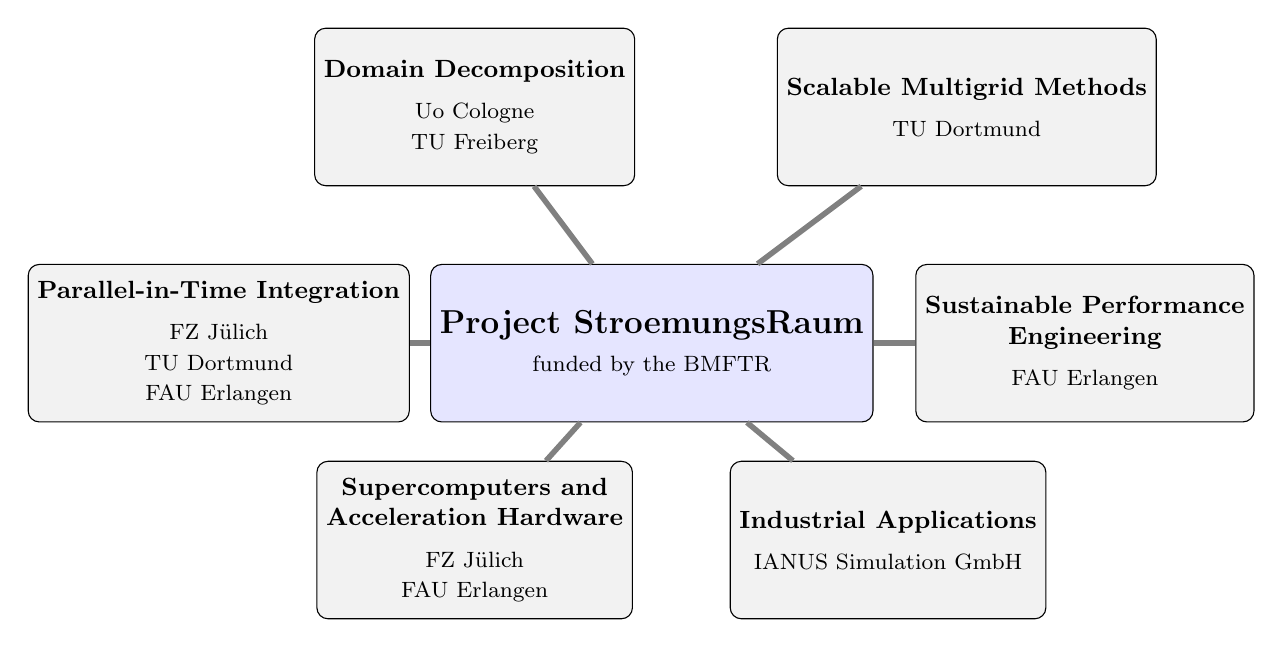
\begin{tikzpicture}[
			% Removed "mindmap" as it applies specific styling that's hard to override
			every node/.style={
					rectangle,
					rounded corners,
					minimum width=2cm,
					minimum height=2cm,
					align=center,
					font=\small,
					text=black,
					draw=black,
					fill=gray!10
				},
			root concept/.style={
					fill=blue!10,
					font=\bfseries\large,
					text=black,
					minimum width=3cm
				},
			% Custom edge style
			conn/.style={
					draw=black!50,
					line width=2pt,
					solid
				},
		]
		\begin{scope}[shift={(-5, 3)}]
			\node[root concept] (root) {Project StroemungsRaum\\{\normalfont\footnotesize funded by the BMFTR}};

			% Create child nodes with explicit positioning and manual edges
			\node[xshift=5.5cm, yshift=0cm] (n1) {\bf{Sustainable Performance}\\\bf{Engineering}\\[1ex]\footnotesize FAU Erlangen};
			\node[xshift=4cm, yshift=3cm] (n2) {\bf{Scalable Multigrid Methods}\\[1ex] \footnotesize TU Dortmund};
			\node[xshift=-2.25cm, yshift=3cm] (n3) {\bf{Domain Decomposition}\\[1ex]\footnotesize \alert{Uo Cologne}\\ \footnotesize TU Freiberg};
			\node[xshift=-5.5cm, yshift=0cm] (n4) {\bf{Parallel-in-Time Integration}\\[1ex] \footnotesize FZ Jülich\\ \footnotesize TU Dortmund\\ \footnotesize FAU Erlangen};
			\node[xshift=-2.25cm, yshift=-2.5cm] (n5) {\bf{Supercomputers and}\\\bf{Acceleration Hardware}\\[1ex] \footnotesize FZ Jülich\\\footnotesize FAU Erlangen};
			\node[xshift=3cm, yshift=-2.5cm] (n6) {\bf{Industrial Applications}\\[1ex] \footnotesize IANUS Simulation GmbH};
			%
			% % Draw thin connections
			\draw[conn] (root) -- (n1);
			\draw[conn] (root) -- (n2);
			\draw[conn] (root) -- (n3);
			\draw[conn] (root) -- (n4);
			\draw[conn] (root) -- (n5);
			\draw[conn] (root) -- (n6);
		\end{scope}
        % \node [inner sep=0pt] at (2,-0.5) {Project Stroemungsraum \includegraphics[width=0.25\textwidth]{images/StroemungsRaumMap.png}};
	\end{tikzpicture}
}

% 	\end{figure}
% \end{frame}

\begin{frame}{Some References on Nonlinear Domain Decomposition Methods}
	\tiny
	\textbf{Nonlinear FETI-DP and Nonlinear BDDC:}\\
	Klawonn, Lanser, Rheinbach (2012, 2013, 2014, 2015, 2016, 2018), Klawonn, Lanser, Rheinbach, Uran (2017, 2018), Klawonn Lanser, Uran (2021, 2023), \dots\\~\\

	\textbf{Nonlinear Elimination:}\\
	Hwang, Lin, Cai (2010); Cai, Li (2011); Wang, Su, Cai (2015); Hwang, Su, Cai (2016); Gong, Cai (2018); Luo, Shiu, Chen, Cai (2019); Gong, Cai (2019); Liu, Hwang, Luo, Cai, Keyes (2022), \dots\\~\\

	\textbf{ASPIN:}\\
	Cai, Keyes 2002; Cai, Keyes, Marcinkowski 2002; Hwang, Cai 2005, 2007; Groß, Krause (2010, 2013), \dots\\~\\

	\textbf{MSPIN and Field-split methods:}\\
	Keyes, Liu, (2015, 2016,2021); Liu, Wei, Keyes (2017); Kopanicáková, Kothari, Krause (2023), \dots\\~\\

	\textbf{RASPEN:}\\
	Dolean, Gander, Kherijii, Kwok, Masson (2016)\\~\\

    \hspace*{-2.7mm}
    \noindent\fcolorbox{red}{white}{
        \begin{minipage}{0.4\textwidth}
            \textbf{Nonlinear 2-Level Schwarz:}\\
			Heinlein, Lanser (2020); Heinlein, Klawonn, Lanser (2022)
		\end{minipage}}\\~\\

	\textbf{Nonlinear Neumann-Neumann:}\\ Bordeu, Boucard, Gosselet 2009\\~\\

	\textbf{Nonlinear FETI-1:}\\
	Pebrel, Rey, Gosselet 2008; Negrello, Gosselet, Rey (2021)\\~\\

	\textbf{Other DD work reversing linearization and decomposition:}\\
	Ganis, Juntunen, Pencheva, Wheeler, Yotov 2014; Ganis, Kumar, Pencheva, Wheeler, Yotov 2014
\end{frame}

\begin{frame}{Two-level nonlinear Schwarz}%: Nonlinearly preconditioned inexact Newton algorithms}}
	\begin{tikzpicture}[transform shape]
    % Define coordinates for the main elements
    \coordinate (leftImg) at (0,0);
    \coordinate (topImg) at (5,2.5);
    \coordinate (bottomImg) at (5,-2.5);
    \coordinate (rightEq) at (10,1.0);
    
    % Place the placeholder images (blue rectangles with numerical solution)
    \node[inner sep=0] (leftRectangle) at (leftImg) 
        {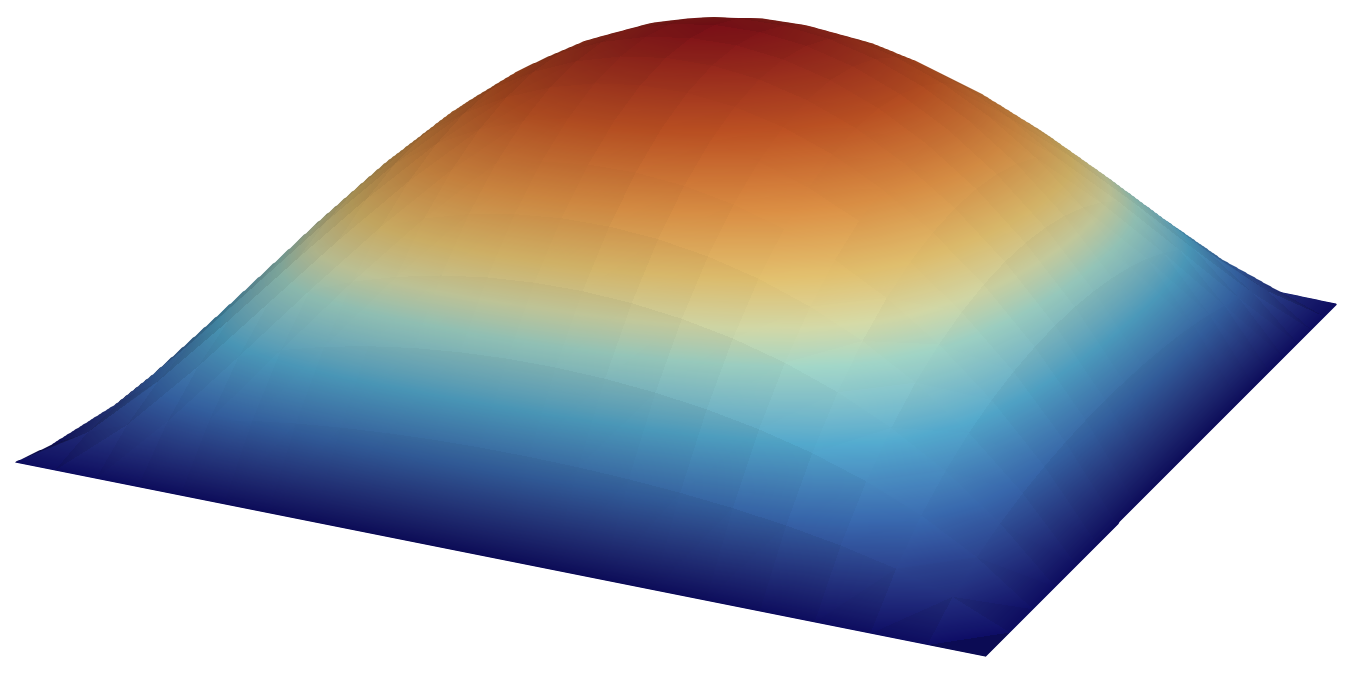
\includegraphics[width=5cm]{images/global-solution.png}};
    \node[inner sep=0] (topRectangle) at (topImg) 
        {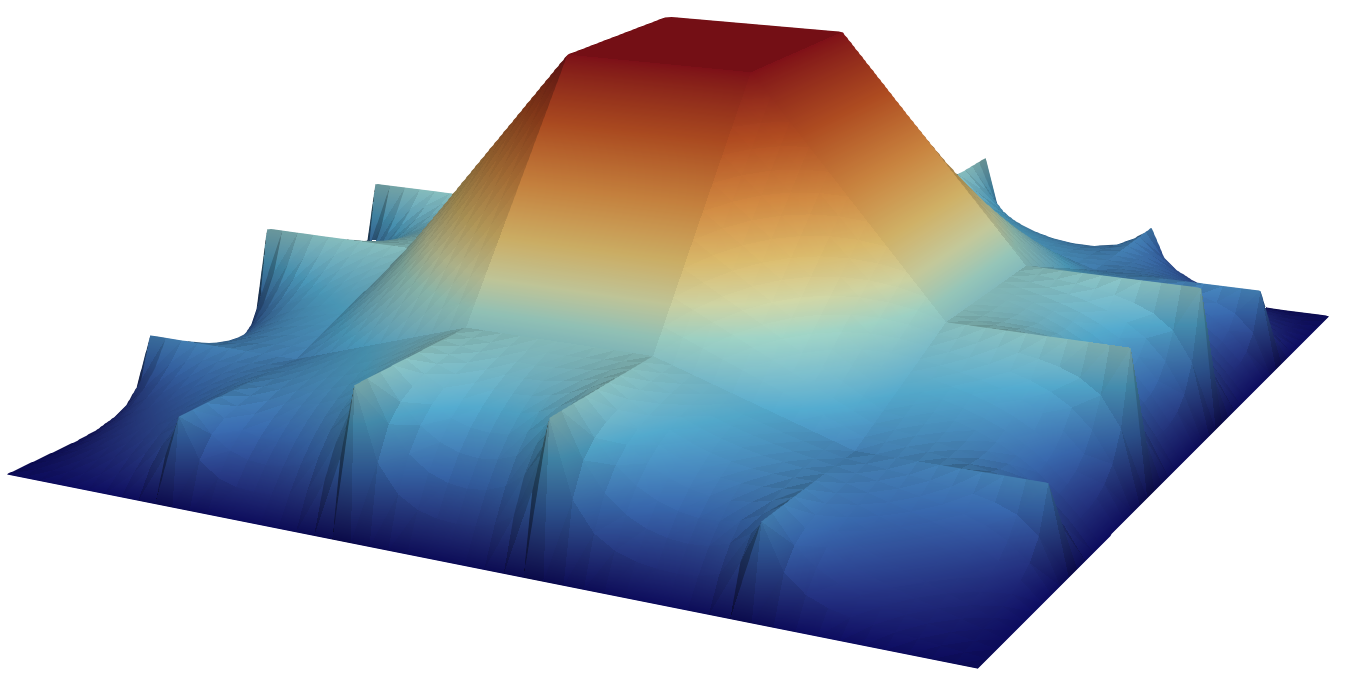
\includegraphics[width=5cm]{images/coarse-solution.png}};
     \node[inner sep=0] (bottomRectangle) at (bottomImg) 
        {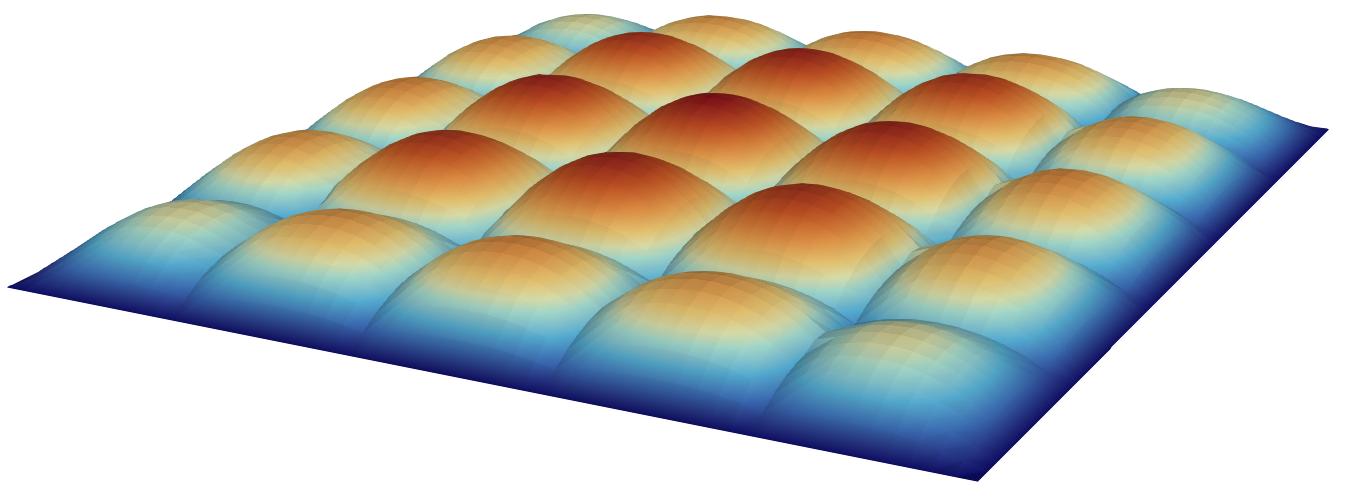
\includegraphics[width=5cm]{images/local-solutions.png}};
    
    \node[fill=white, fill opacity=0.7, text opacity=1, yshift=5mm, xshift=2mm, text width = 35mm] at (leftRectangle.north) {\small Discretized nonlinear problem};
    \node[yshift=0cm, fill=white, fill opacity=0.9, text opacity=1] at (leftRectangle.south) {\small $F(u) = 0$};

    \node[yshift=0cm, fill=white, fill opacity=0.9, text opacity=1] at (bottomRectangle.south) {\small $R_i F\left(\bm{u} - R_i^T T_i(\bm{u})\right) = 0$};
    
    \node [fill=white, fill opacity=0.9, text opacity=1] at (topRectangle.south){\small $\Phi^T F\left(\bm{u} - \Phi T_0(\bm{u})\right) = 0$};
    
    \node[align=left, fill=white, fill opacity=0.7, text opacity=1, text width = 4.5cm] at (9.6,-1.3){\small Solve with Newton's method for nonlinear corrections $T_i(u), \quad i = 0,\ldots, N$};
    
    \node[draw, rectangle, minimum width=4cm, minimum height=1cm] (boxedEq) at (rightEq) {\small $\mathcal{F}(\bm{u}) = \sum_{i=0}^{N} R_i^T T_i(\bm{u})$};
    
    % Arrows
    \draw[-{Stealth[length=3mm, width=2mm]}] ($(leftRectangle.north east) + (-0.5, -0.5)$) -- ($(topRectangle.south west) + (0.3, 0.3)$);
    \draw[-{Stealth[length=3mm, width=2mm]}] ($(leftRectangle.south east) + (-0.7, 0.4)$) -- ($(bottomRectangle.north west) + (0.8, -0.2)$);
    \draw[-{Stealth[length=3mm, width=2mm]}] ($(topRectangle.south east)+ (-0.3, 0.7)$) -- ($(boxedEq.north west)+ (-0.1, 0.1)$);
    \draw[-{Stealth[length=3mm, width=2mm]}] ($(bottomRectangle.north east)+ (-0.8, -0.1)$) -- ($(boxedEq.south west)+ (-0.1, -0.1)$);
\end{tikzpicture}

\end{frame}

\begin{frame}{Software ecosystem}
	\begin{tikzpicture}[node distance = 1cm, auto]

	\node [whtblock,text depth=14mm] (FEDDLIB) {
		{\footnotesize \textbf{FEDDLib}\textsuperscript{a}} \\[0.3em] \tiny \textbf{F}inite \textbf{E}lement and \textbf{D}omain \textbf{D}ecomposition \textbf{Lib}rary
		\begin{itemize}
			\item{Parallel finite element assembly}
			\item{Specific problem definition}
			\item{Mesh handling routines}
			      % \item \textcolor{orange}{Update two-level nonlinear Schwarz solver for elasticity and Navier-Stokes}
			      % \item \textcolor{orange}{Test with various coarse spaces}
		\end{itemize}
		% \hspace*{-25mm}\scalebox{.7}{By University of Cologne, TU Delft, TU Freiberg}
	};

	\node [whtblock, right=of FEDDLIB,node distance=7cm, rectangle split part fill={orange!20,blue!5},] (FeatFlow) {
		{ \footnotesize\textbf{FEAT3}\textsuperscript{b}}\\[0.3em] \tiny Finite element based solution of incompressible\\Navier-Stokes in 2D and 3D
		\vspace{2pt}
		\begin{itemize}
			%\setlength{\itemsep}{0pt}
			\item \textcolor{red}{Interface with \texttt{FROSch}}
			\item \textcolor{red}{Test (non-Newtonian, high Reynolds, exascale)}
		\end{itemize}};

	%===============================================    
	\node [whtblock, below=of FEDDLIB, text depth=18mm, node distance=3.5cm,] (Trilinos) {
		{\footnotesize \textbf{Trilinos}\textsuperscript{c}}
		\begingroup
		\addtolength{\leftmargini}{0.5cm}
		\vspace{1pt}
		\tiny
		\begin{itemize}
			%\setlength{\itemsep}{0pt}
			\item Data services: Vectors, matrices, graphs and related operations
			\item Linear and Eigenproblem solvers
			\item Nonlinear solvers and analysis tools
		\end{itemize}
		\endgroup
	};

	\node[inner sep=0pt] (trilinos_logo) at ([xshift=6mm, yshift=0mm] Trilinos.west){
\includegraphics[width=.125\textwidth, angle=90,origin=c]{images/logo/Trilinos_logo_new.png}};

	\node [whtblock, text depth=18mm, right=of Trilinos,node distance=7cm,rectangle split part fill={orange!20,blue!5},] (Frosch) {
		{\footnotesize \textbf{FROSch}\textsuperscript{d}} \\[0.4em]  \hspace{6em}\tiny\textbf{F}ast and \textbf{R}obust \textbf{O}verlapping \textbf{S}chwarz
		\vspace*{0.5em}
		\begingroup
		\addtolength{\leftmargini}{4em}
		\begin{itemize}
			\item \textcolor{red}{Implement two-level nonlinear Schwarz solver}
			\item \textcolor{red}{Test with various coarse spaces on various model problems}
		\end{itemize}
		\endgroup
	};

	\node[inner sep=0pt] (trilinos_logo) at ([xshift=7.5mm, yshift=0mm] Frosch.west){
\includegraphics[width=.1\textwidth]{images/logo/FROSch_logo.png}};

	%%%%%%%%%%%%%%%%%%%%%%%%%%%%%%%%
	%   CONTAINERS -- BACKGROUND LIGHT-DASHED BLOCKS
	%%%%%%%%%%%%%%%%%%%%%%%%%%%%%%%%
	\begin{scope}[on background layer]

		\coordinate (aux2) at ([yshift=0mm]Trilinos.north);
		\node[container2, fit=(aux2) (Trilinos) (Frosch)] (Trilinos_blue) {};

		\coordinate (aux3) at ([yshift=0mm] FeatFlow.north);
		\node[container3, fit=(aux3) (FeatFlow)] (FeatFlow_Green) {};

		\coordinate (aux1) at ([yshift=0mm]FEDDLIB.north);
		\node [container,fit=(aux1) (FEDDLIB)] (FEDDLIB_ORANGE) {};
		\node at ([yshift=0.7mm]Trilinos_blue.north) [fill=gray!10,draw,minimum width=8em,minimum height=1em] (FEDTRI-label) {\footnotesize\textbf{Interface}};

	\end{scope}
	%************************************************************
	%************************************************************
	%  Draw edges
	%************************************************************
	%************************************************************
	% \path [line,thick] (FEDDLIB) -- (FEDTRI-label);
	% \path [line,thick] (Trilinos) -- (Frosch);
	% \path [line,thick] (FEDTRI-label) -- (Trilinos);
	% \path [line,red,thick] (FeatFlow) -- (FEDTRI-label);

\end{tikzpicture}
\tiny\\~\\

a: University of Cologne, TU Delft, TU Freiberg (https://github.com/FEDDLib/FEDDLib.git)\\
b: TU Dortmund (https://github.com/tudo-math-ls3/feat3)\\
c: Sandia National Laboratories (https://trilinos.github.io)\\
d: University of Cologne, TU Delft, TU Freiberg (https://shylu-frosch.github.io)\\

\end{frame}




\section{Hyperelasticity}
\begin{frame}{2D compressible plane-stress neo-Hookean material}
	\vspace{0mm}
	\begin{columns}
		\begin{column}{0.4\textwidth}%
			\begin{align*}
				\label{eq:nonlinelas}
				\begin{split}
					-\mathrm{div}(P(F)) = f_{vol}\; & \mathrm{in}\;\Omega,           \\
					u = g_D \;                      & \mathrm{on}\;\partial\Omega_D, \\
					n\cdot P(F) = g_N\;             & \mathrm{on}\;\partial\Omega_N,
				\end{split}
			\end{align*}
			\begin{figure}
				\centering
				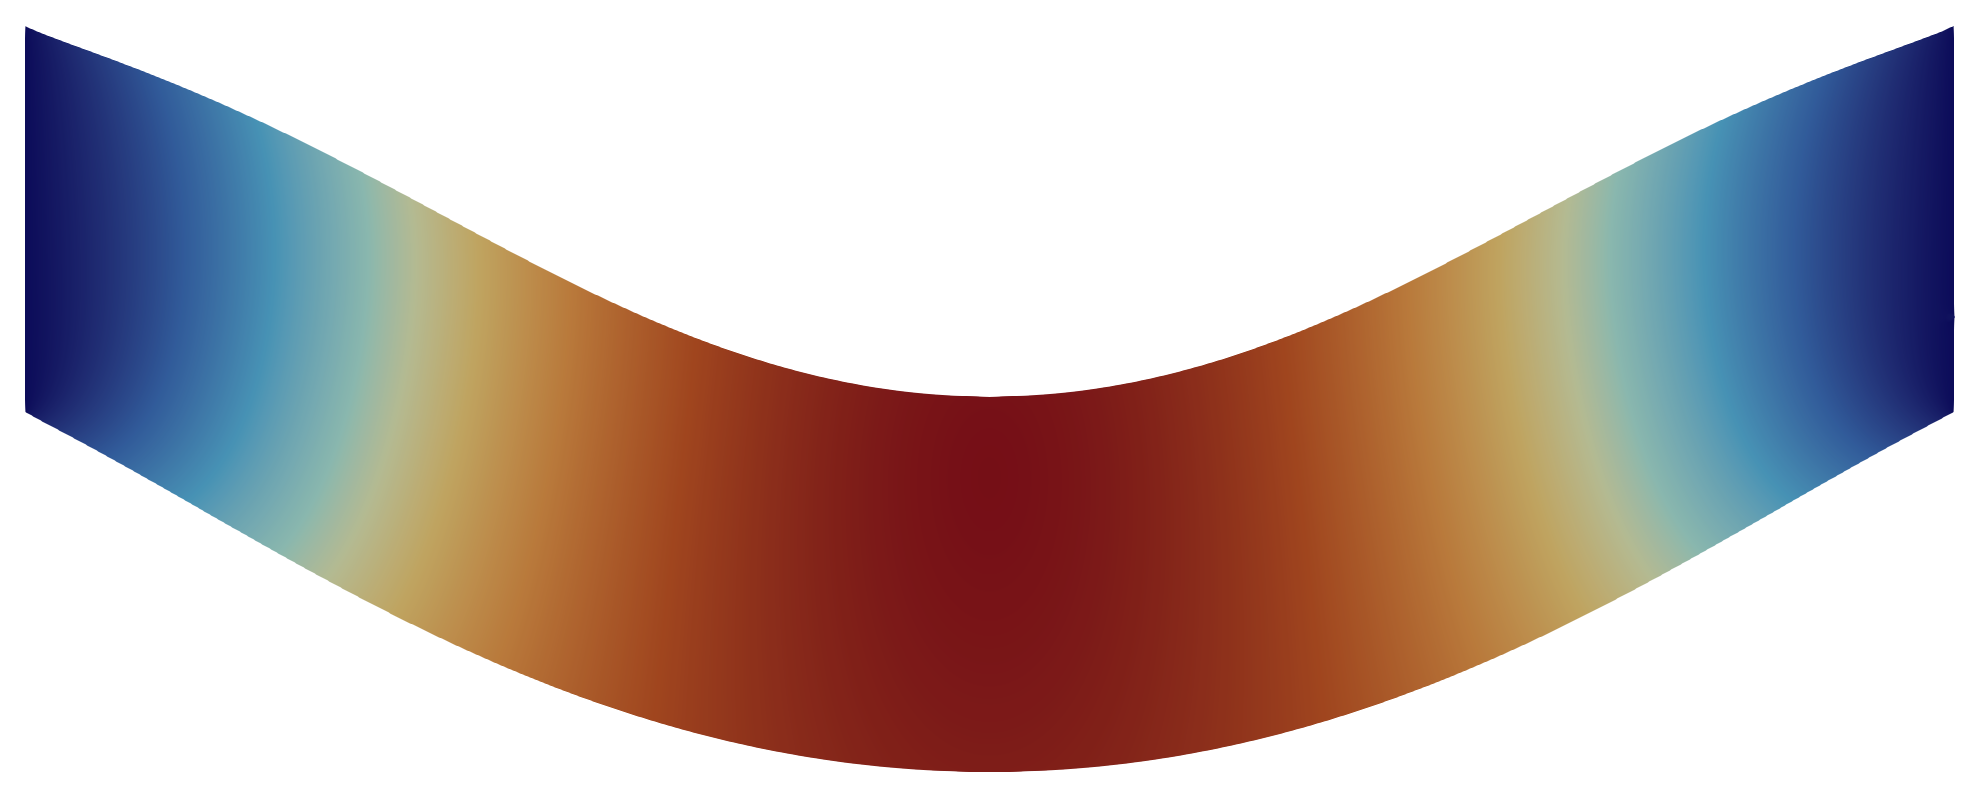
\includegraphics[width=0.9\textwidth]{images/beam2D.png}
				\caption{2D beam with applied volume force.}
				\label{fig:beam2d}
			\end{figure}
		\end{column}%
		\begin{column}{0.6\textwidth}
			\vspace{-1em}
			\centering
			\begin{itemize}
				% \setlength{\itemsep}{15pt}
				\item $F$ Deformation gradient
				\item $P(F) = \frac{E}{1(1+\nu)}(F-F^{-T}) + \frac{E\nu}{(1+\nu)(1-2\nu)}\mathrm{ln}(\mathrm{det}(F)F^{-T})$
				\item $\nu$ = 0.3
				\item $E$ = 210 GPa
				\item $5\textrm{m}\times 1\textrm{m}$ 2D mesh with \numgru{2572710} nodes
        \item $g_D = 0$ on short edges
				\item $g_N = 0$ on long edges
				\item P1 elements
        \item Solver relative tolerance: $10^{-4}$
        \item MsFEM coarse space \footnotemark{}
				% \item $f_{vol} = (0,-f_y)$
			\end{itemize}
		\end{column}
	\end{columns}
  \footnotetext{\tiny Dohrmann, Widlund (2017)}
\end{frame}

\begin{frame}{Strong scaling: nonlinear elasticity}
	\begin{itemize}
		\item $f_y = 4$ MN/m$^{2}$
	\end{itemize}
	\begin{figure}
		\centering
		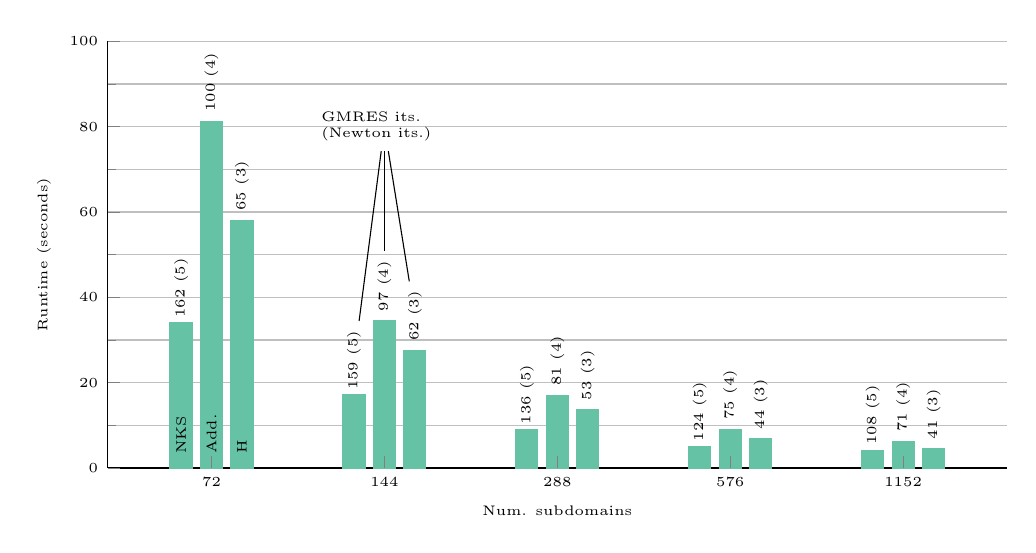
\begin{tikzpicture}
	\pgfplotsset{
		every axis/.append style={
				ybar stacked,
				width=13cm,
				height=7cm,
				ylabel={Runtime (seconds)},
				xlabel={Num. subdomains},
				symbolic x coords={72, 144, 288, 576, 1152},
				xtick=data,
				enlarge x limits=0.15,
				legend style={at={(1,1)},anchor=north east},
				axis lines*=left, ymajorgrids, yminorgrids,
				ymin=0,
				ymax=100,
				bar width=8pt,
				minor y tick num=1,
				xticklabel style={rotate=0,xshift=0ex,anchor=north},
				cycle list name=Set2-5,
			},
		% Ensures that bars are plotted full
		every axis plot/.append style={
				fill,
			},
	}
	\tikzstyle{mynodestyle} = [rotate=90, anchor=west]

	% Solver = H1
	\begin{axis}[bar shift=11pt, hide axis]
		% Another option for relative node placement
		% \node [left=11pt of 256.base, anchor=base] {test}; % Custom number above bar for 256
		\node[mynodestyle] at ([xshift=11pt]axis cs:72,58) {$65$ $(3)$};
		\node[mynodestyle] (one) at ([xshift=11pt]axis cs:144,27.5) {$62$ $(3)$};
		\node[mynodestyle] at ([xshift=11pt]axis cs:288,13.6){$53$ $(3)$};
		\node[mynodestyle] at ([xshift=11pt]axis cs:576,6.8){$44$ $(3)$};
		\node[mynodestyle] at ([xshift=11pt]axis cs:1152,4.5){$41$ $(3)$};
		\node [mynodestyle](oneRe) at ([xshift=11pt]axis cs:72,1) {H};

		\addplot coordinates {(72,58) (144,27.5) (288,13.6) (576,6.8) (1152,4.5)};
	\end{axis}

	% Solver = Add.
	\begin{axis}[bar shift=0pt, hide axis]
		\node[mynodestyle] at (axis cs:72,81.2) {$100$ $(4)$};
		\node[mynodestyle](two) at (axis cs:144,34.5) {$97$ $(4)$};
		\node[mynodestyle]at (axis cs:288,17) {$81$ $(4)$};
		\node[mynodestyle]at (axis cs:576,9) {$75$ $(4)$};
		\node[mynodestyle]at (axis cs:1152,6.2) {$71$ $(4)$};
		\node [mynodestyle]at (axis cs:72,1) {Add.};

		\addplot+ coordinates {(72,81.2) (144,34.5) (288,16.9) (576,9) (1152,6.2)};
	\end{axis}

	% Solver = NKS

	\begin{axis}[bar shift=-11pt]
		%% Overlap = 10
		% \node [mynodestyle] at([xshift=-11pt]axis cs:72,42) {$190$ $(5)$};
		% \node [mynodestyle](three) at([xshift=-11pt]axis cs:144,22.5) {$200$ $(5)$};
		% \node [mynodestyle]at([xshift=-11pt]axis cs:288,11.8) {$170$ $(5)$};
		% \node [mynodestyle]at([xshift=-11pt]axis cs:576,7.3) {$150$ $(5)$};
		% \node [mynodestyle]at([xshift=-11pt]axis cs:1152,5.2) {$135$ $(5)$};
		% \node [mynodestyle]at ([xshift=-11pt]axis cs:72,1) {NKS};
		%
		% \addplot+ coordinates {(72,41.7) (144,22.5) (288,11.8) (576,7.3) (1152,5.2)};


		%% Overlap = 5
		\node [mynodestyle]at([xshift=-11pt]axis cs:72,33) {$162$ $(5)$};
		\node [mynodestyle](three) at([xshift=-11pt]axis cs:144,16) {$159$ $(5)$};
		\node [mynodestyle]at([xshift=-11pt]axis cs:288,8) {$136$ $(5)$};
		\node [mynodestyle]at([xshift=-11pt]axis cs:576,4) {$124$ $(5)$};
		\node [mynodestyle]at([xshift=-11pt]axis cs:1152,3.2) {$108$ $(5)$};
		\node [mynodestyle]at([xshift=-11pt]axis cs:72,1) {NKS};

		\addplot+ coordinates {(72,34) (144,17.1) (288,9.1) (576,5.1) (1152,4.2)};
		\node[text width=1.6cm] (gmres) at (axis cs:144,80){GMRES its. (Newton its.)};

	\end{axis}

	\draw [thin] (gmres) --  (one);
	\draw [thin] (gmres) --  (two);
	\draw [thin] (gmres) --  (three);

\end{tikzpicture}

		\label{fig:strong-scalability-elascticity}
	\end{figure}
\end{frame}

\begin{frame}{Newton-Krylov-Schwarz vs nonlinear Schwarz}
	\begin{itemize}
		\item $576$ Subdomains
	\end{itemize}
	\begin{figure}
		\centering
		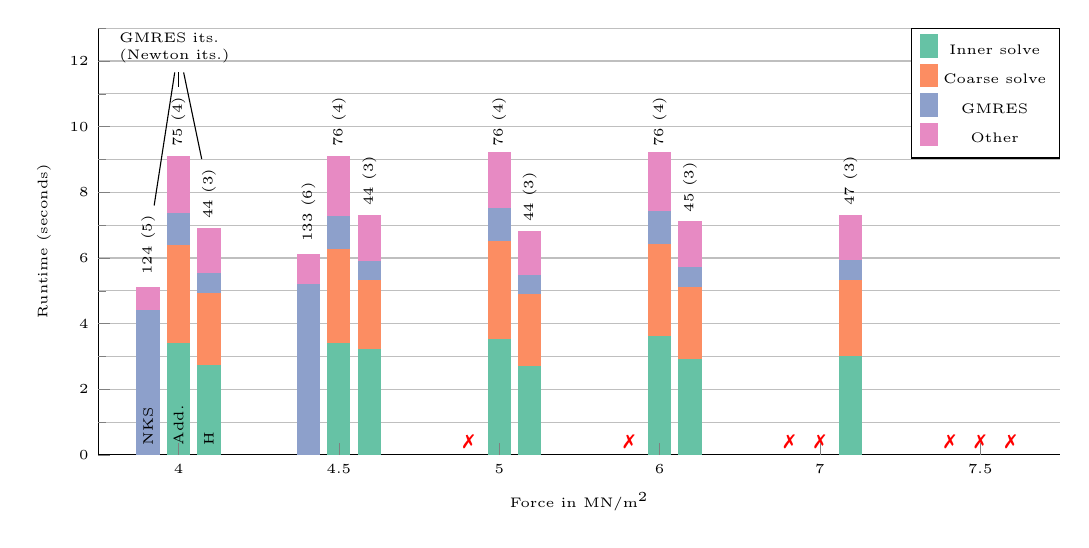
\begin{tikzpicture}
	\pgfplotsset{
		every axis/.append style={
				legend style={at={(1,1)},anchor=north east},
				axis lines*=left, ymajorgrids, yminorgrids,
				width=13.8cm, height=7cm,
				ymin=0,
				ymax=13,
				ybar stacked,
				bar width=8pt,
				minor y tick num=1,
				symbolic x coords={1,2,3,4,5,6},
				xtick={1,2,3,4,5,6},
				xticklabels from table={\hybrid}{Force},
				xticklabel style={rotate=0,xshift=0ex,anchor=north},
				ylabel={Runtime (seconds)},
				xlabel={Force in MN/m$^{2}$},
				cycle list name=Set2-5,
			},
		every axis plot/.append style={fill},
	}

	\tikzstyle{mynodestyle} = [rotate=90, anchor=west]

	\pgfplotstableread{
		Location Force  GlobalSolve   InnerSolve   CoarseSolve   GMRES    Other
		1        4      6.9           2.73         2.2           0.58     1.39
		2        4.5    7.3           3.2          2.1           0.59     1.41
		3        5      6.8           2.7          2.2           0.57     1.33
		4        6      7.1           2.9          2.2           0.61     1.39
		5        7      7.3           3            2.3           0.61     1.39
		6        7.5    0             0            0             0        0
	}\hybrid

	\pgfplotstableread{
		Location Force  GlobalSolve   InnerSolve   CoarseSolve   GMRES    Other
		1        4      9.1           3.38         3             0.96     1.76
		2        4.5    9.1           3.4          2.85          1        1.85
		3        5      9.2           3.5          3             1        1.7
		4        6      9.2           3.6          2.8           1        1.8
		5        7      0             0            0             0        0
		6        7.5    0             0            0             0        0
	}\RGDSWtwo
 
  %% Overlap = 10
	% \pgfplotstableread{
	% 	Location Force  GlobalSolve   GMRES    Other
	% 	1        4      7.2           6.5      0.7
	% 	2        4.5    8.2           7.4      0.8
	% 	3        5      0             0        0
	% 	4        6      0             0        0
	% 	5        7      0             0        0
	% 	6        7.5    0             0        0
	% }\NKS

  %% Overlap = 5
	\pgfplotstableread{
		Location Force  GlobalSolve   GMRES    Other
		1        4      5.1           4.4      0.7
		2        4.5    6.1           5.2      0.9
		3        5      0             0        0
		4        6      0             0        0
		5        7      0             0        0
		6        7.5    0             0        0
	}\NKS

	\begin{axis}[bar shift=0pt, hide axis]
		\node[mynodestyle]at (axis cs:1,0) {Add.};
		\node[mynodestyle] (two) at (axis cs:1,9.1) {$75$ $(4)$};
		\node[mynodestyle] at(axis cs:2,9.1) {$76$ $(4)$};
		\node[mynodestyle] at(axis cs:3,9.1) {$76$ $(4)$};
		\node[mynodestyle] at(axis cs:4,9.1) {$76$ $(4)$};
		\node at(axis cs:5,.4) {\scriptsize\color{red}\ding{55}};
		\node at(axis cs:6,.4) {\scriptsize\color{red}\ding{55}};

		\addplot+ table [x=Location, y=InnerSolve] {\RGDSWtwo};
		\addplot+ table [x=Location, y=CoarseSolve] {\RGDSWtwo};
		\addplot+ table [x=Location, y=GMRES] {\RGDSWtwo};
		\addplot+ table [x=Location, y=Other] {\RGDSWtwo};
	\end{axis}

	\begin{axis}[bar shift=11pt]
		\node[mynodestyle] at ([xshift=11pt]axis cs:1,0) {H};
		\node[xshift=11pt,mynodestyle] (three) at (axis cs:1,6.9) {$44$ $(3)$};
		\node[xshift=11pt,mynodestyle] at (axis cs:2,7.3) {$44$ $(3)$};
		\node[xshift=11pt,mynodestyle] at (axis cs:3,6.8) {$44$ $(3)$};
		\node[xshift=11pt,mynodestyle] at (axis cs:4,7.1) {$45$ $(3)$};
		\node[xshift=11pt,mynodestyle] at (axis cs:5,7.3) {$47$ $(3)$};
		\node[xshift=11pt,rotate=0] at  (axis cs:6,.4) {\scriptsize\color{red}\ding{55}};

		\addplot+ table [y=InnerSolve] {\hybrid}; \addlegendentry{Inner solve}
		\addplot+ table [y=CoarseSolve] {\hybrid}; \addlegendentry{Coarse solve}
		\addplot+ table [y=GMRES] {\hybrid}; \addlegendentry{GMRES}
		\addplot+ table [y=Other] {\hybrid}; \addlegendentry{Other}
	\end{axis}

	\begin{axis}[bar shift=-11pt, hide axis, cycle list shift=2]
		\node[mynodestyle]at ([xshift=-11pt]axis cs:1,0) {NKS};
		\node[xshift=-11pt,mynodestyle] (one) at (axis cs:1,5.2) {$124$ $(5)$};
		\node[xshift=-11pt,mynodestyle] at (axis cs:2,6.2) {$133$ $(6)$};
		\node[xshift=-11pt,rotate=0] at (axis cs:3,.4) {\scriptsize\color{red}\ding{55}};
		\node[xshift=-11pt,rotate=0] at (axis cs:4,.4) {\scriptsize\color{red}\ding{55}};
		\node[xshift=-11pt,rotate=0] at (axis cs:5,.4) {\scriptsize\color{red}\ding{55}};
		\node[xshift=-11pt,rotate=0] at (axis cs:6,.4) {\scriptsize\color{red}\ding{55}};
		\node[text width=1.5cm] (gmres) at (axis cs:1,12.4) {GMRES its. (Newton its.)};

		\addplot+ table [x=Location, y=GMRES] {\NKS};
		\addplot+ table [x=Location, y=Other] {\NKS};
	\end{axis}

	\draw [thin] (gmres) --  (one);
	\draw [thin] (gmres) --  (two);
	\draw [thin] (gmres) --  (three);

\end{tikzpicture}

		\label{fig:nks-vs-nls}
	\end{figure}
\end{frame}

 \begin{frame}{Summary nonlinear elasticity}
   \begin{itemize}
     \item Strong scaling of two-level nonlinear Schwarz variants is on-par with NKS.
     \item Two-level nonlinear Schwarz variants are more robust against nonlinearity.
   \end{itemize}
 \end{frame}


\section{Lid-driven cavity}
\begin{frame}{Stationary and dimensionless Navier-Stokes equations}
	\vspace{-5mm}
	\begin{columns}
		\begin{column}{0.6\textwidth}%
			\begin{align*}
				-\frac{1}{\rm Re} \Delta v + (v \cdot \nabla)v + \nabla p & = 0 \;   & {\rm in}\; \Omega           \\
				{\rm div}(v)                                              & = 0 \;   & {\rm in} \; \Omega          \\
				v                                                         & = v_0 \; & {\rm on} \; \partial \Omega
			\end{align*}
			\vspace{-4mm}
			\begin{itemize}
				\item $v_0=(1,0)$ on the lid and zero everywhere else
				\item $\mathcal{P}$1-$\mathcal{P}$1-Stab (Bochev-Dohrmann) \footnotemark{}
				\item Subdomain size: $150\times 150$ elements
				\item Solver absolute and relative tolerances: \num{e-6}
				\item RGDSW coarse space
				\item Hybrid variant
			\end{itemize}
		\end{column}
		\begin{column}{0.4\textwidth}
			\begin{figure}
				\centering
				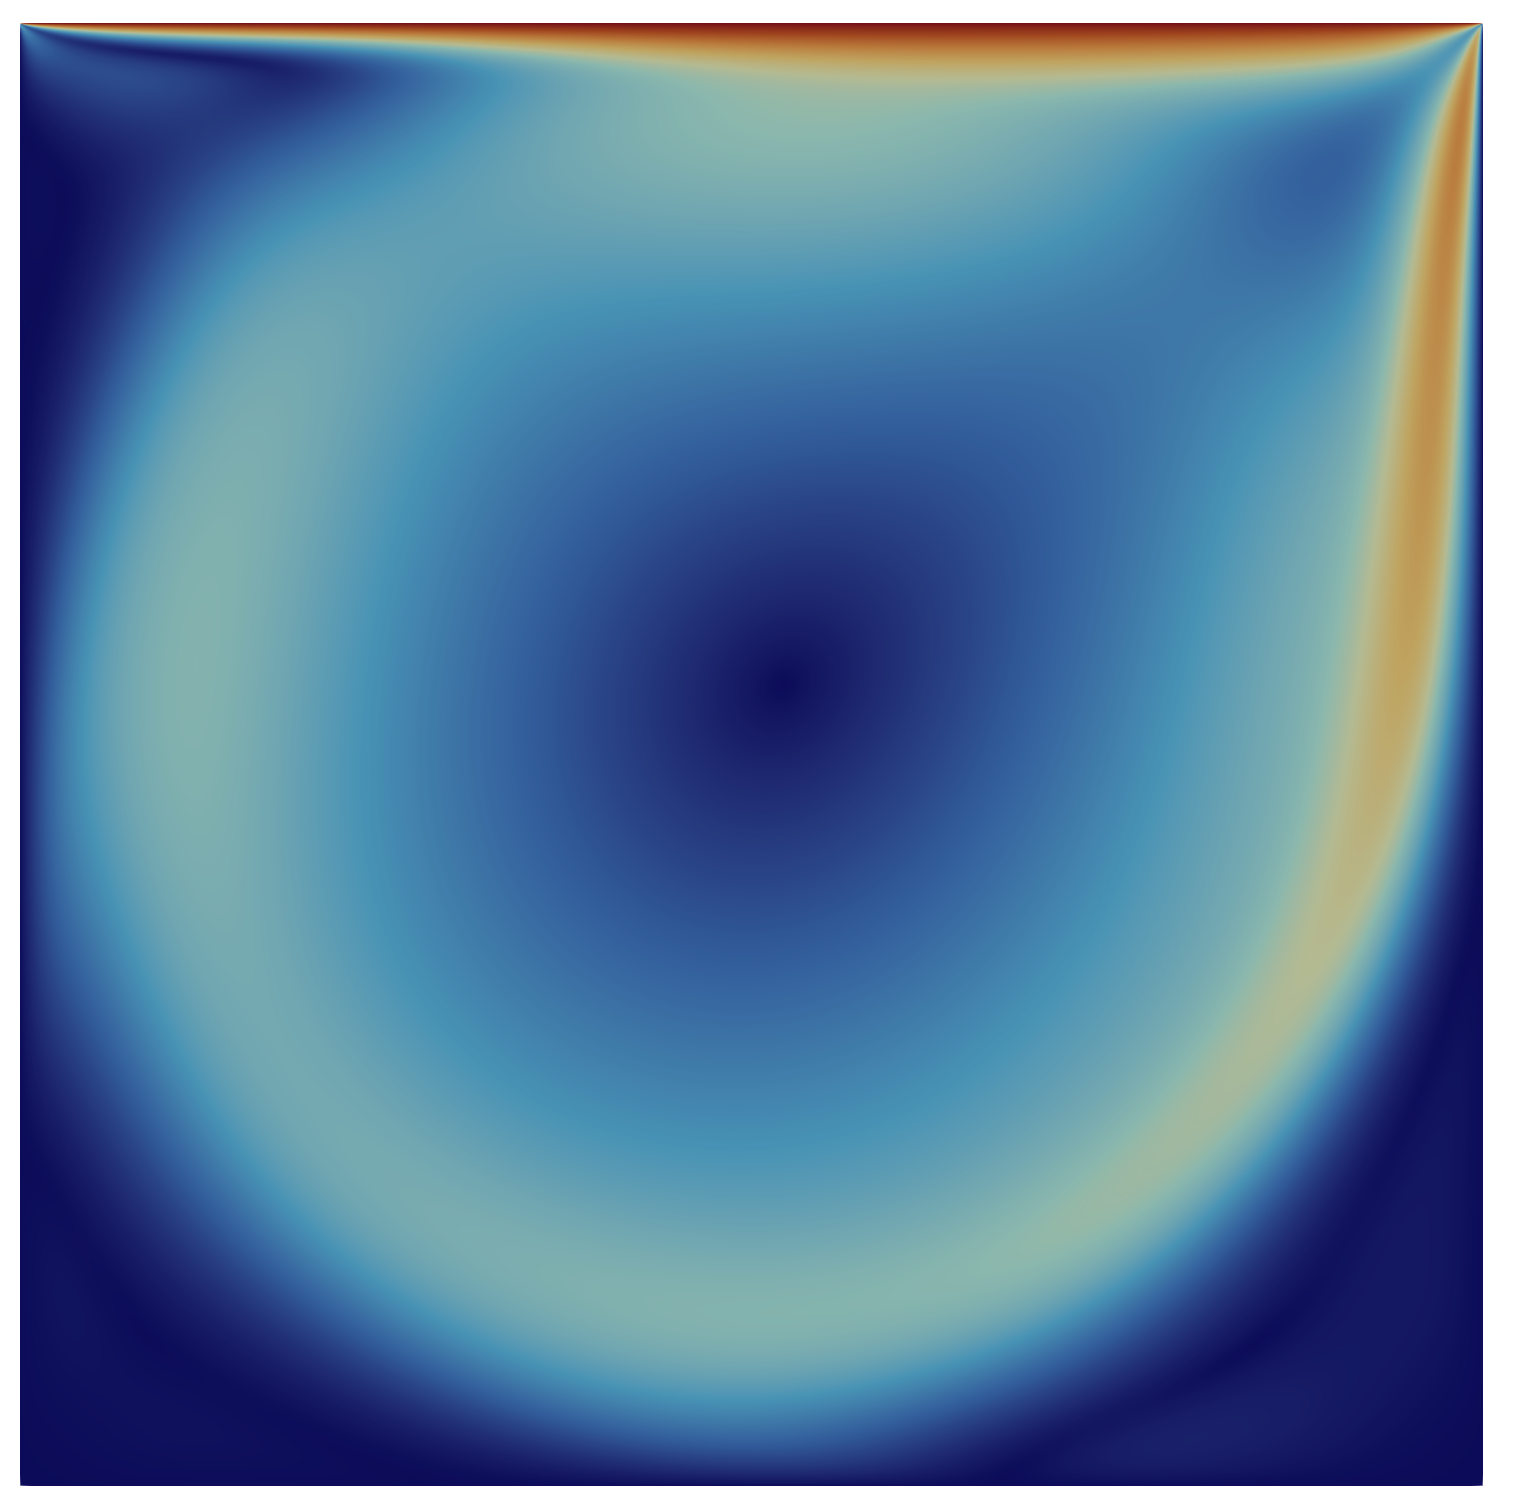
\includegraphics[width=0.7\textwidth]{images/ldc.png}
				\caption{Lid-driven cavity}
			\end{figure}
		\end{column}
	\end{columns}
	\footnotetext{\tiny Bochev, Dohrmann (2004)}
\end{frame}

\begin{frame}{Lid-driven cavity: nonlinear Schwarz weak scalability}
	\begin{figure}
		\centering
		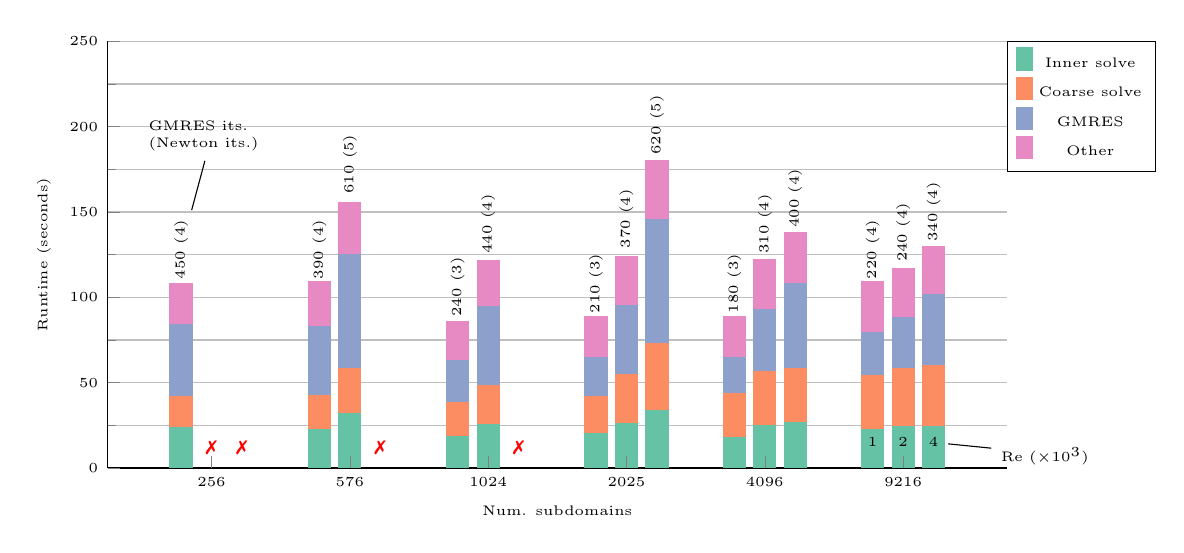
\begin{tikzpicture}
	\pgfplotsset{
		every axis/.append style={
				ybar stacked,
				width=13cm,
				height=7cm,
				ylabel={Runtime (seconds)},
				xlabel={Num. subdomains},
				symbolic x coords={256, 576, 1024, 2025, 4096, 9216},
				xtick=data,
				enlarge x limits=0.15,
				legend style={at={(1,1)},anchor=north west},
				axis lines*=left, ymajorgrids, yminorgrids,
				ymin=0,
				ymax=250,
				bar width=8pt,
				minor y tick num=1,
				xticklabel style={rotate=0,xshift=0ex,anchor=north},
				cycle list name=Set2-5,
			},
		% Ensures that bars are plotted full
		every axis plot/.append style={
				fill,
			},
	}
  \tikzstyle{mynodestyle} = [rotate=90, anchor=west]

	% Re = 1000
	\begin{axis}[bar shift=-11pt, hide axis]
		% Another option for relative node placement
		% \node [left=11pt of 256.base, anchor=base] {test}; % Custom number above bar for 256
		\node[mynodestyle] (one) at ([xshift=-11pt]axis cs:256,105) {$450$ $(4)$};
		\node[mynodestyle] at ([xshift=-11pt]axis cs:576,105) {$390$ $(4)$};
		\node[mynodestyle] at ([xshift=-11pt]axis cs:1024,83){$240$ $(3)$};
		\node[mynodestyle] at ([xshift=-11pt]axis cs:2025,85){$210$ $(3)$};
		\node[mynodestyle] at ([xshift=-11pt]axis cs:4096,85){$180$ $(3)$};
		\node[mynodestyle] at ([xshift=-11pt]axis cs:9216,105){$220$ $(4)$};
		\node (oneRe) at ([xshift=-11pt]axis cs:9216,15) {$1$};

        \addplot coordinates  {(256,23.8 ) (576,  22.8 ) (1024, 18.3 ) (2025, 20	) (4096, 17.9)  (9216,22.6  )};   
        \addplot+ coordinates {(256,18.3 ) (576,  19.9 ) (1024, 19.8 ) (2025, 22	) (4096, 25.9)  (9216,31.3)}; 
        \addplot+ coordinates {(256,42.2 ) (576,  40.3 ) (1024, 25 )   (2025, 22.8	) (4096, 20.7)  (9216,25.5)};   
        \addplot+ coordinates {(256,23.7 ) (576,  26   ) (1024, 22.8 ) (2025, 23.9	) (4096, 24.1)  (9216,29.6)}; 







    \end{axis}

	% Re = 2000
	\begin{axis}[bar shift=0pt, hide axis]

		\node[rotate=0] at (axis cs:256,12) {\scriptsize\color{red}\ding{55}};
		\node[mynodestyle](576) at (axis cs:576,155) {$610$ $(5)$};
		\node[mynodestyle](1024) at (axis cs:1024,120) {$440$ $(4)$};
		\node[mynodestyle](2025) at (axis cs:2025,123) {$370$ $(4)$};
		\node[mynodestyle](4096) at (axis cs:4096,120) {$310$ $(4)$};
		\node[mynodestyle](9216) at (axis cs:9216,115) {$240$ $(4)$};
		\node at (axis cs:9216,15) {$2$};


        \addplot coordinates  {(256, 0)     (576,32.1) (1024, 25.2) (2025, 25.8) (4096, 24.8)  (9216,24  )};
        \addplot+ coordinates {(256, 0)     (576,26.4) (1024, 23.4) (2025, 28.7) (4096, 31.7)  (9216,34.5)};
        \addplot+ coordinates {(256, 0)     (576,66.4) (1024, 46  ) (2025, 40.7) (4096, 36.1)  (9216,29.4  )};
        \addplot+ coordinates {(256, 0)     (576,30.7) (1024, 26.8) (2025, 28.8) (4096, 29.4)  (9216,29.1)};
	\end{axis}

	% Re = 4000
	\begin{axis}[bar shift=11pt]

		\node[xshift=11pt,rotate=0] at (axis cs:256,12) {\scriptsize\color{red}\ding{55}};
		\node[xshift=11pt,rotate=0] at (axis cs:576,12) {\scriptsize\color{red}\ding{55}};
		\node[xshift=11pt,rotate=0] at (axis cs:1024,12) {\scriptsize\color{red}\ding{55}};
		\node [mynodestyle]at([xshift=11pt]axis cs:2025,178) {$620$ $(5)$};
		\node [mynodestyle]at([xshift=11pt]axis cs:4096,135) {$400$ $(4)$};
		\node [mynodestyle]at([xshift=11pt]axis cs:9216,127) {$340$ $(4)$};
		\node(fourRe) at ([xshift=11pt]axis cs:9216,15) {$4$};

        \addplot+ coordinates { (256, 0) (576, 0) (1024, 0) (2025,33.8) (4096,26.6) (9216,24.4)}; 
        \addplot+ coordinates { (256, 0) (576, 0) (1024, 0) (2025,39)  (4096,31.7)  (9216,35.7)};   
        \addplot+ coordinates { (256, 0) (576, 0) (1024, 0) (2025,72.5) (4096,50)   (9216,41.4)};  
        \addplot+ coordinates { (256, 0) (576, 0) (1024, 0) (2025,34.7) (4096,29.7) (9216,28.5)}; 

    \node[anchor=south,text width=1.6cm] (gmres) at (axis cs:256,180){GMRES its. (Newton its.)};

		\legend{
			Inner solve,
			Coarse solve,
			GMRES,
			Other
		}

	\end{axis}

	\node[rotate=0, text width=1.8cm] (Re) at ([yshift=-5,xshift=50]fourRe){Re ($\times 10^{3}$)};

	% \draw [thin] (gmres) --  (256);
	\draw [thin] (gmres) --  (one);
	% \draw [thin] (gmres) --  (three);

	\draw [thin] (Re) --  (fourRe);

\end{tikzpicture}

		\label{fig:weak-scalability-nls}
	\end{figure}
\end{frame}

\begin{frame}{Lid-driven cavity: nonlinear Schwarz weak scalability}
	\begin{figure}
		\centering
		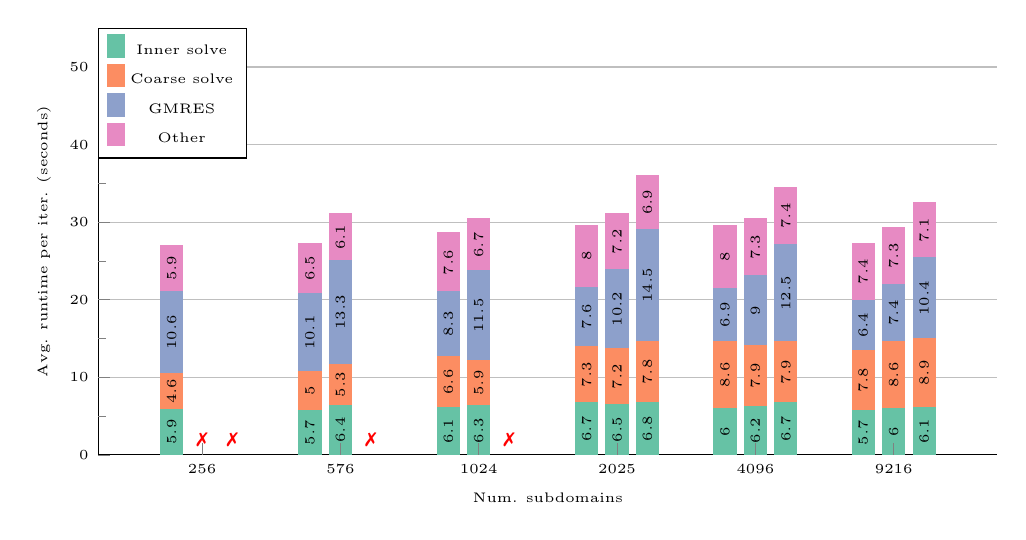
\begin{tikzpicture}
	\pgfplotsset{
		every axis/.append style={
				ybar stacked,
				width=13cm,
				height=7cm,
				ylabel={Avg. runtime per iter. (seconds)},
				xlabel={Num. subdomains},
				symbolic x coords={256, 576, 1024, 2025, 4096, 9216},
				xtick=data,
				enlarge x limits=0.15,
				legend style={at={(0,1)},anchor=north west},
				axis lines*=left, ymajorgrids,
				ymin=0,
				ymax=55,
				bar width=8pt,
				nodes near coords,
				nodes near coords style={rotate=90},
				minor y tick num=1,
				xticklabel style={rotate=0,xshift=0ex,anchor=north},
				cycle list name=Set2-5,
			},
		% Ensures that bars are plotted full
		every axis plot/.append style={
				fill,
				% fill opacity=0.5,
				every node/.append style={
						text=black,
					},
			},
	}
	% Re = 1000

	\begin{axis}[bar shift=-11pt, hide axis]
		\addplot+ coordinates {(256,5.9  ) (576, 5.7	 ) (1024,   6.1) (2025,  6.7 ) (4096, 6) (9216,5.7 )};
		\addplot+ coordinates {(256,4.6 ) (576, 5 )  (1024,  6.6 ) (2025,  7.3 ) (4096, 8.6 )    (9216,7.8)};
		\addplot+ coordinates {(256,10.6 ) (576, 10.1)  (1024,  8.3 ) (2025,  7.6 ) (4096, 6.9 ) (9216,6.4  )};
		\addplot+ coordinates {(256,5.9 ) (576, 6.5	 ) (1024,   7.6) (2025,  8) (4096, 8   )     (9216,7.4 )};
	\end{axis}

	% Re = 2000
	\begin{axis}[bar shift=0pt, hide axis]

		\node[rotate=0] at (axis cs:256,2) {\scriptsize\color{red}\ding{55}};
		\addplot+ coordinates {(256, 0) (576,6.4 ) (1024, 6.3	) (2025,  6.5   )  (4096,  6.2   ) (9216,6   )};
		\addplot+ coordinates {(256, 0) (576,5.3 ) (1024, 5.9  ) (2025,  7.2  ) (4096,  7.9 )      (9216,8.6)};
		\addplot+ coordinates {(256, 0) (576,13.3) (1024, 11.5  ) (2025,  10.2 ) (4096,  9 )       (9216,7.4  )};
		\addplot+ coordinates {(256, 0) (576,6.1 ) (1024, 6.7	) (2025,  7.2	 )  (4096,  7.3  ) (9216,7.3)};
	\end{axis}

	% Re = 4000
	\begin{axis}[bar shift=11pt]

		\node[xshift=11pt,rotate=0] at (axis cs:256,2) {\scriptsize\color{red}\ding{55}};
		\node[xshift=11pt,rotate=0] at (axis cs:576,2) {\scriptsize\color{red}\ding{55}};
		\node[xshift=11pt,rotate=0] at (axis cs:1024,2) {\scriptsize\color{red}\ding{55}};

		\addplot+ coordinates {(256,0) (576,0) (1024,0)  (2025,  6.8) (4096, 6.7  )   (9216,6.1 )};
		\addplot+ coordinates {(256,0) (576,0) (1024,0)  (2025,  7.8 ) (4096, 7.9)    (9216,8.9  )};
		\addplot+ coordinates {(256,0) (576,0) (1024,0)  (2025,  14.5) (4096, 12.5  ) (9216,10.4)};
		\addplot+ coordinates {(256,0) (576,0) (1024,0)  (2025,  6.9) (4096, 7.4)     (9216,7.1)};

		\legend{
			Inner solve,
			Coarse solve,
			GMRES,
			Other
		}
	\end{axis}
\end{tikzpicture}

		\label{fig:weak-scalability-per-iter-nls}
	\end{figure}
\end{frame}

\begin{frame}{LDC: Newton-Krylov-Schwarz vs Hybrid, 256 subdomains}
	\begin{figure}
		\centering
		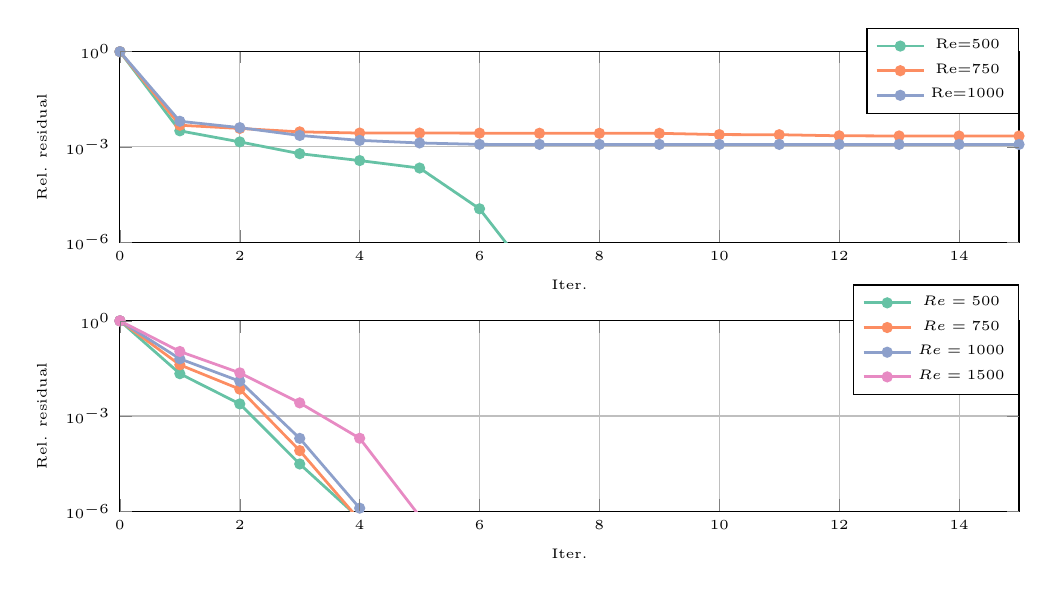
\begin{tikzpicture}
    \begin{groupplot}[
        group style={group size=1 by 2, vertical sep=1.cm},
        width=13cm, height=4cm,
        xlabel={Iter.},
        grid=major,
        log basis y=10,
        legend style={at={(1.0,0.9)},anchor=east},
				xmin=0,
				xmax=15,
				ymin=1e-6,
				ymax=1,
        every axis plot/.append style={line width=1pt, mark size=1.5pt, mark=*},
    ]
    \nextgroupplot[
        ylabel={Rel. residual},
        ymode=log,
    ]
    \addplot coordinates {
        (0, 1) (1, 0.00320133) (2, 0.00143493) (3, 0.000610389) 
        (4, 0.000369944) (5, 0.000215426) (6, 1.11767e-05) (7, 4.18693e-08)
    };
    \addlegendentry{Re=500}
    \addplot coordinates {
        (0, 1) (1, 0.00480191) (2, 0.00380737) (3, 0.00297334)
        (4, 0.00272655) (5, 0.00272013) (6, 0.00270843) (7, 0.00268613)
        (8, 0.00267774) (9, 0.00266959) (10, 0.00243689) (11, 0.0024165)
        (12, 0.00223072) (13, 0.00221035) (14, 0.002201) (15, 0.00219758)
        (16, 0.00219347) (17, 0.00219139) (18, 0.00219044) (19, 0.00219027)
        (20, 0.00218816) (21, 0.00218768) (22, 0.0021868) (23, 0.00218531)
        (24, 0.00218251) (25, 0.00217408) (26, 0.00217307) (27, 0.00217296)
        (28, 0.00217293) (29, 0.00217293)
    };
    \addlegendentry{Re=750}
    \addplot coordinates {
        (0, 1) (1, 0.00640242) (2, 0.00404174) (3, 0.00228814)
        (4, 0.00160117) (5, 0.00132757) (6, 0.00119772) (7, 0.00119687)
        (8, 0.00119643) (9, 0.00119643) (10, 0.00119643) (11, 0.00119643)
        (12, 0.00119643) (13, 0.00119643) (14, 0.00119643) (15, 0.00119643)
        (16, 0.00119643) (17, 0.00119643) (18, 0.00119643) (19, 0.00119643)
        (20, 0.00119643) (21, 0.00119643) (22, 0.00119643) (23, 0.00119643)
        (24, 0.00119643) (25, 0.00119643) (26, 0.00119643) (27, 0.00119643)
        (28, 0.00119643) (29, 0.00119643)
    };
    \addlegendentry{Re=1000}


    % Absolute residual plot
    \nextgroupplot[
        ylabel={Rel. residual},
        ymode=log,
    ]
    \addplot coordinates {
        (0, 1) (1, 0.0216039) (2, 0.00240872) (3, 3.08805e-05) (4, 5.87615e-07)
    };
    \addlegendentry{$Re=500$}

    \addplot coordinates {
        (0, 1) (1, 0.0410675) (2, 0.00701551) (3, 8.12889e-05) (4, 5.1786e-07)
    };
    \addlegendentry{$Re=750$}

    % \pgfplotsset{cycle list shift=1}
    \addplot coordinates {
        (0, 1) (1, 0.0635524) (2, 0.0125035) (3, 0.000197537) (4, 1.25259e-06)
    };
    \addlegendentry{$Re=1000$}

    \addplot coordinates {
        (0, 1) (1, 0.10807) (2, 0.0229372) (3, 0.0025968) (4, 0.00019946) (5, 7.0061e-07)
    };
    \addlegendentry{$Re=1500$}
    \end{groupplot}
\end{tikzpicture}

		\label{fig:residual-ldc-256}
	\end{figure}
\end{frame}

\begin{frame}{LDC: Newton-Krylov-Schwarz vs Hybrid, 4096 subdomains}
	\begin{figure}
		\centering
		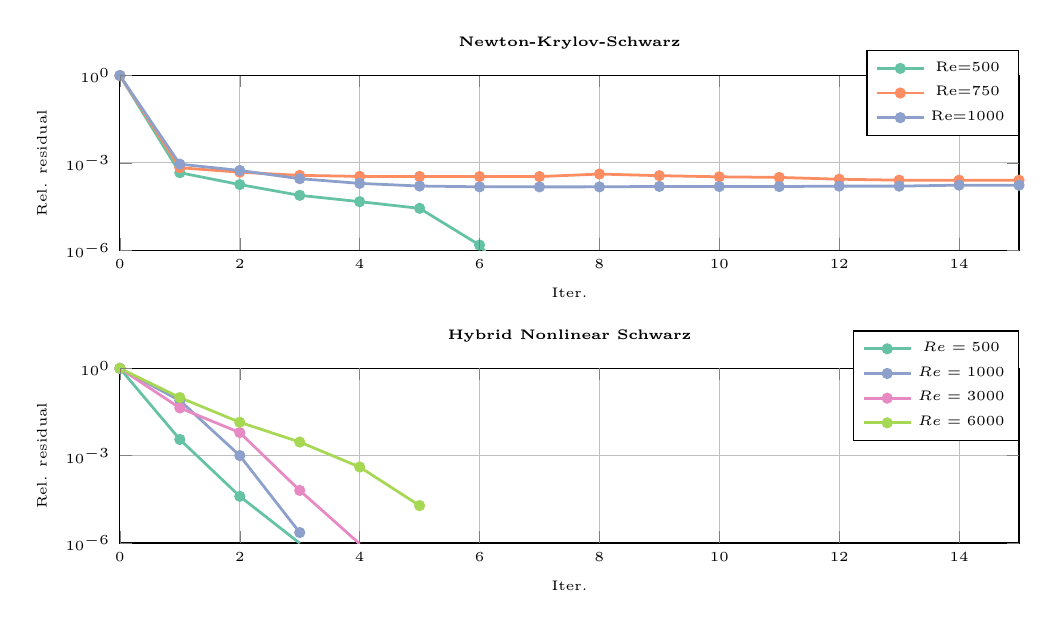
\begin{tikzpicture}
	\begin{groupplot}[
			group style={group size=1 by 2, vertical sep=1.5cm},
			width=13cm, height=3.8cm,
			xlabel={Iter.},
			grid=major,
			log basis y=10,
			legend style={at={(1.0,0.9)},anchor=east},
			xmin=0,
			xmax=15,
			ymin=1e-6,
			ymax=1,
			every axis plot/.append style={line width=1pt, mark size=1.5pt, mark=*},
		]
		\nextgroupplot[
			ylabel={Rel. residual},
            title={\bf{Newton-Krylov-Schwarz}},
			ymode=log,
		]
		\addplot coordinates {
				(0, 1) (1, 0.000461063) (2, 0.000180623) (3, 7.69231e-05) (4, 4.67144e-05) (5, 2.75539e-05) (6, 1.50771e-06) (7, 6.3394e-09)
			};
		\addlegendentry{Re=500}
		\addplot coordinates {
				(0, 1) (1, 0.000683264) (2, 0.000480095) (3, 0.00037343) (4, 0.000345118) (5, 0.000341495) (6, 0.000339957) (7, 0.000339534) (8, 0.000414796) (9, 0.000364827) (10, 0.000333536) (11, 0.000317937) (12, 0.000275248) (13, 0.000256005) (14, 0.000254507) (15, 0.000254237) (16, 0.000262081) (17, 0.00025798) (18, 0.000261379) (19, 0.000260608)
			};
		\addlegendentry{Re=750}
		\addplot coordinates {
            (0, 1) (1, 0.000907096) (2, 0.000549946) (3, 0.000287238) (4, 0.000198314) (5, 0.000160798) (6, 0.000151072) (7, 0.000150393) (8, 0.000150489) (9, 0.000155954) (10, 0.000154682) (11, 0.000154337) (12, 0.000159684) (13, 0.000159413) (14, 0.000172403) (15, 0.000172074) (16, 0.000172708) (17, 0.000189149) (18, 0.000190431) (19, 0.000198664) 
			};
		\addlegendentry{Re=1000}


		% Absolute residual plot
		\nextgroupplot[
			ylabel={Rel. residual},
            title={\bf{Hybrid Nonlinear Schwarz}},
			ymode=log,
		]
		\addplot coordinates {
				(0, 1) (1, 0.00361003) (2, 4.0282e-05) (3, 9.87625e-07)
			};
		\addlegendentry{$Re=500$}

		\pgfplotsset{cycle list shift=1}
		\addplot coordinates {
				(0, 1) (1, 0.0783692) (2, 0.00100882) (3, 2.29151e-06)
			};
		\addlegendentry{$Re=1000$}

		\pgfplotsset{cycle list shift=1}
		\addplot coordinates {
				(0, 1) (1, 0.0436383) (2, 0.00622051) (3, 6.42127e-05) (4, 9.38152e-07)
			};
		\addlegendentry{$Re=3000$}

		\addplot coordinates {
				(0, 1) (1, 0.0994514) (2, 0.0140707) (3, 0.00294689) (4, 0.000409486) (5, 1.93227e-05)
			};
		\addlegendentry{$Re=6000$}
	\end{groupplot}
\end{tikzpicture}

		\label{fig:residual-ldc-4096}
	\end{figure}
\end{frame}

\begin{frame}{Lid-driven cavity coarse basis functions}
	\begin{figure}
		\centering
		\begin{subfigure}{0.5\textwidth}
			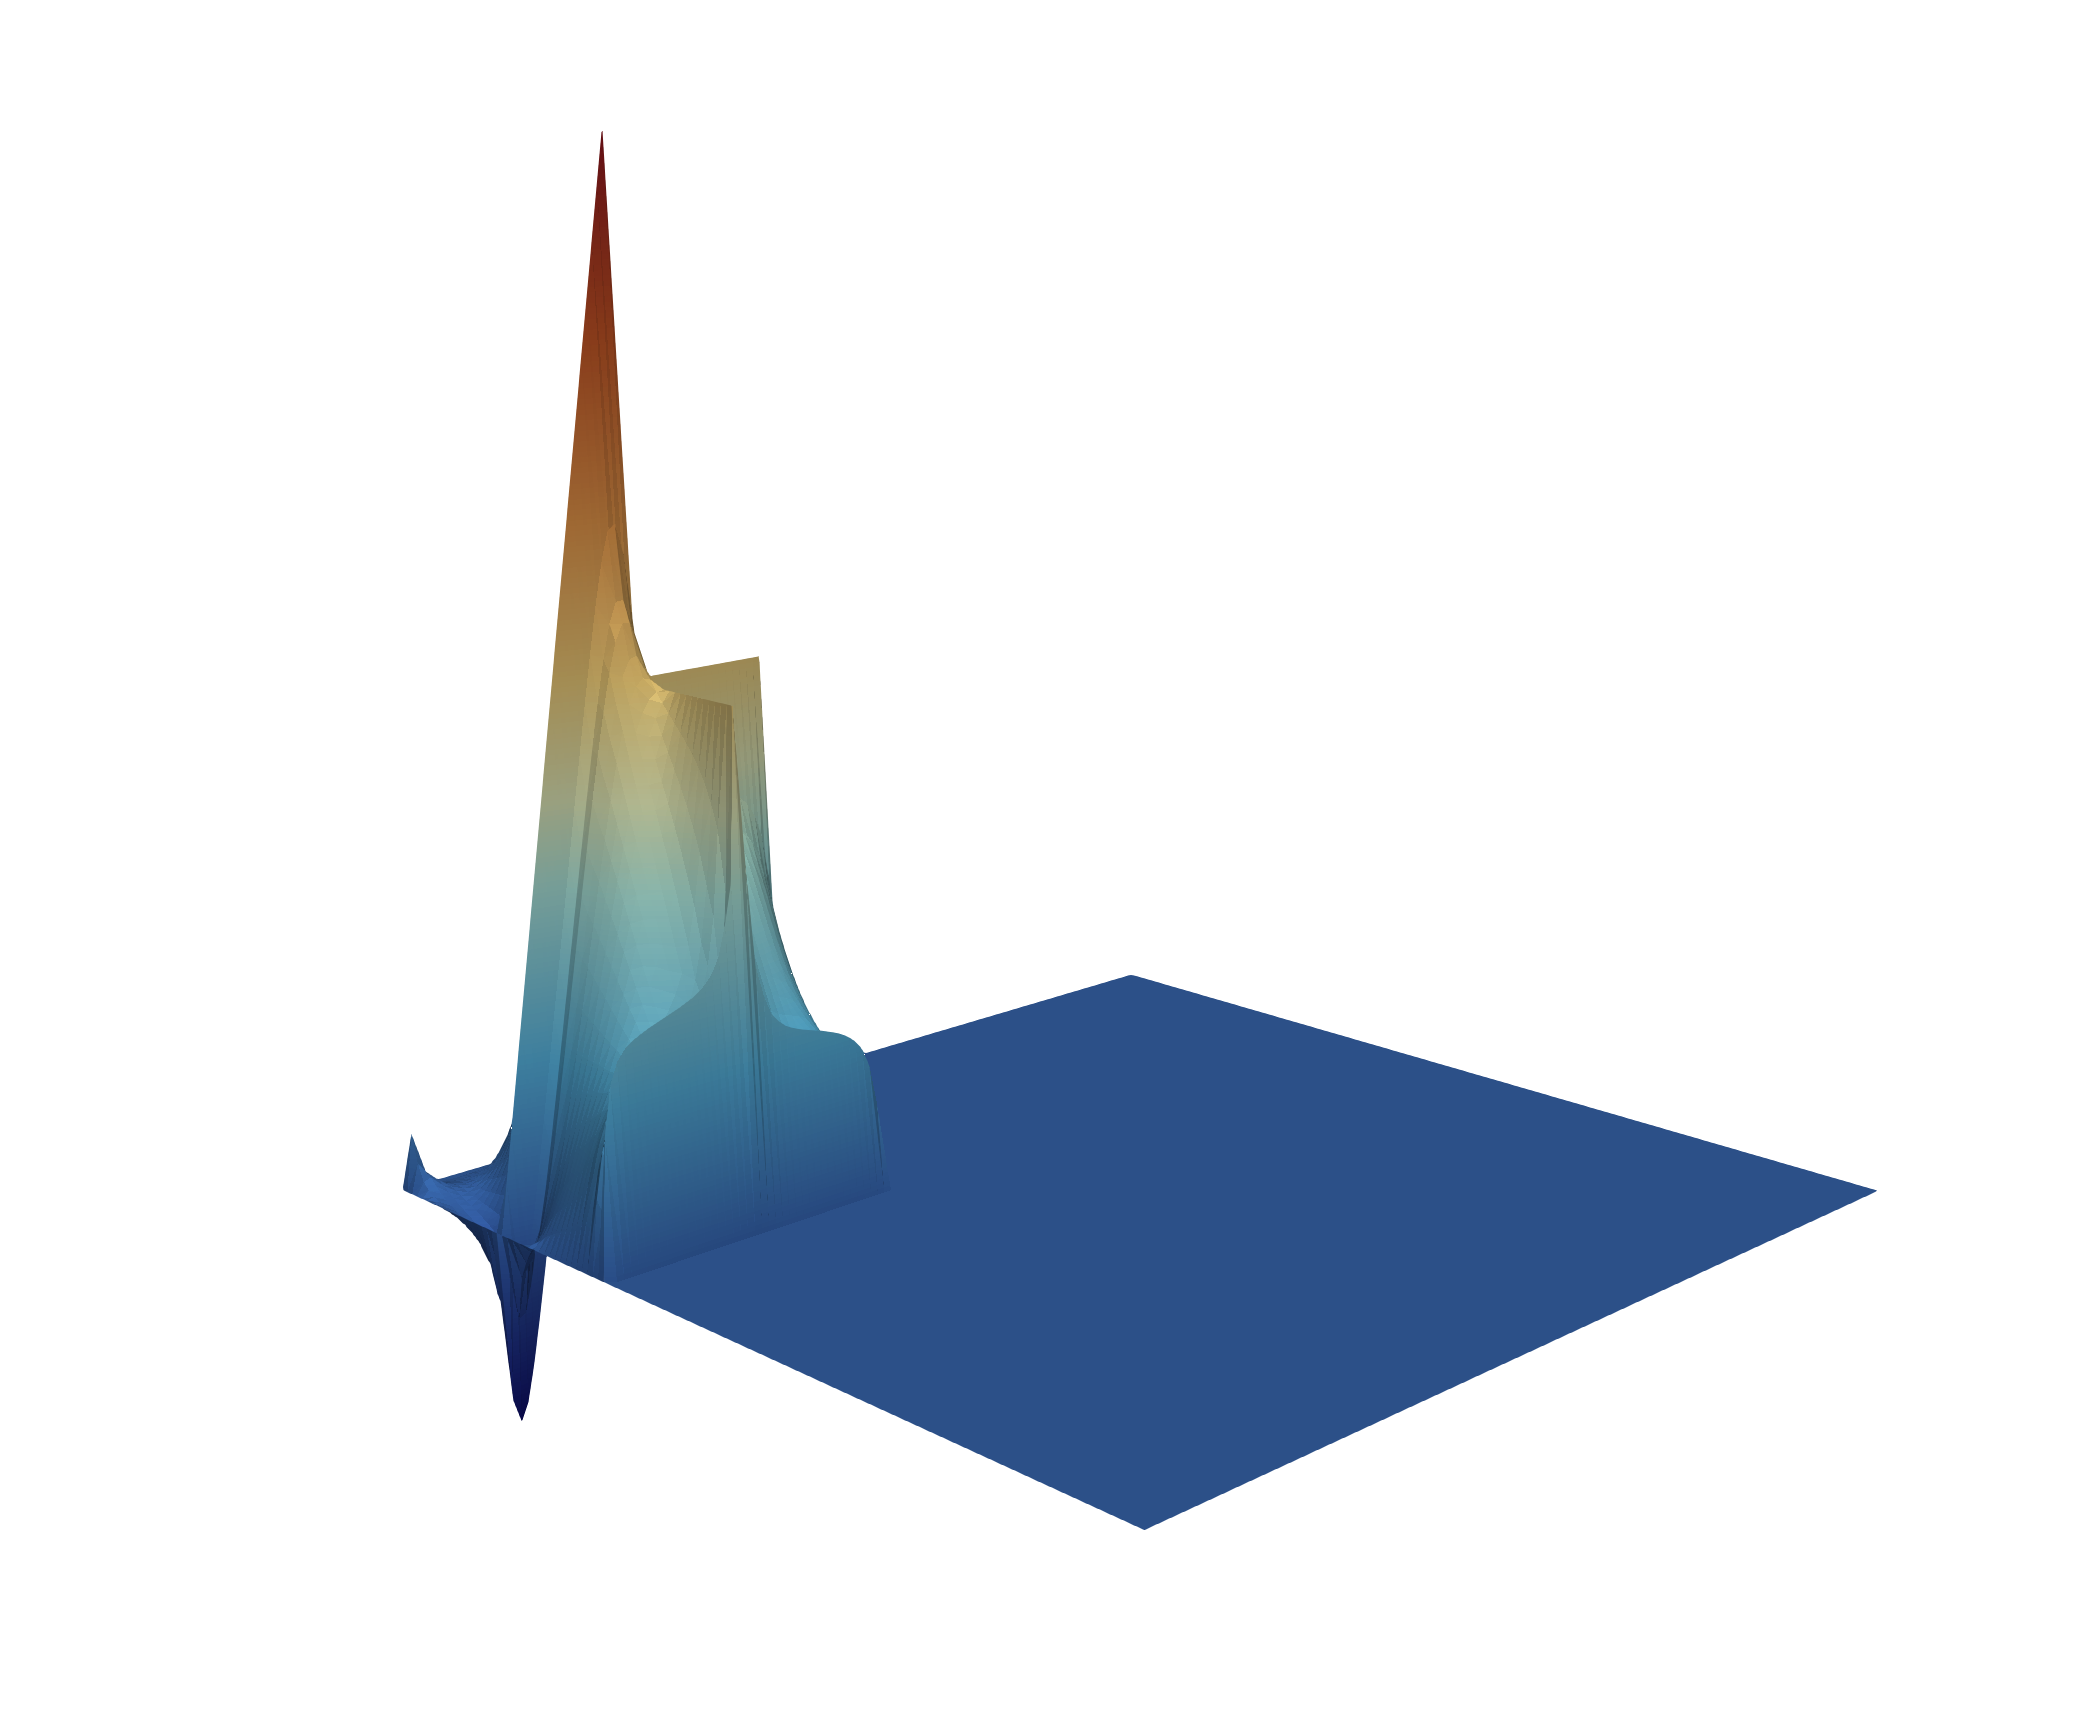
\includegraphics[width=\textwidth]{images/RGDSW-x}
			\caption{RGDSW $x$-component.}
		\end{subfigure}%
		\begin{subfigure}{0.5\textwidth}
			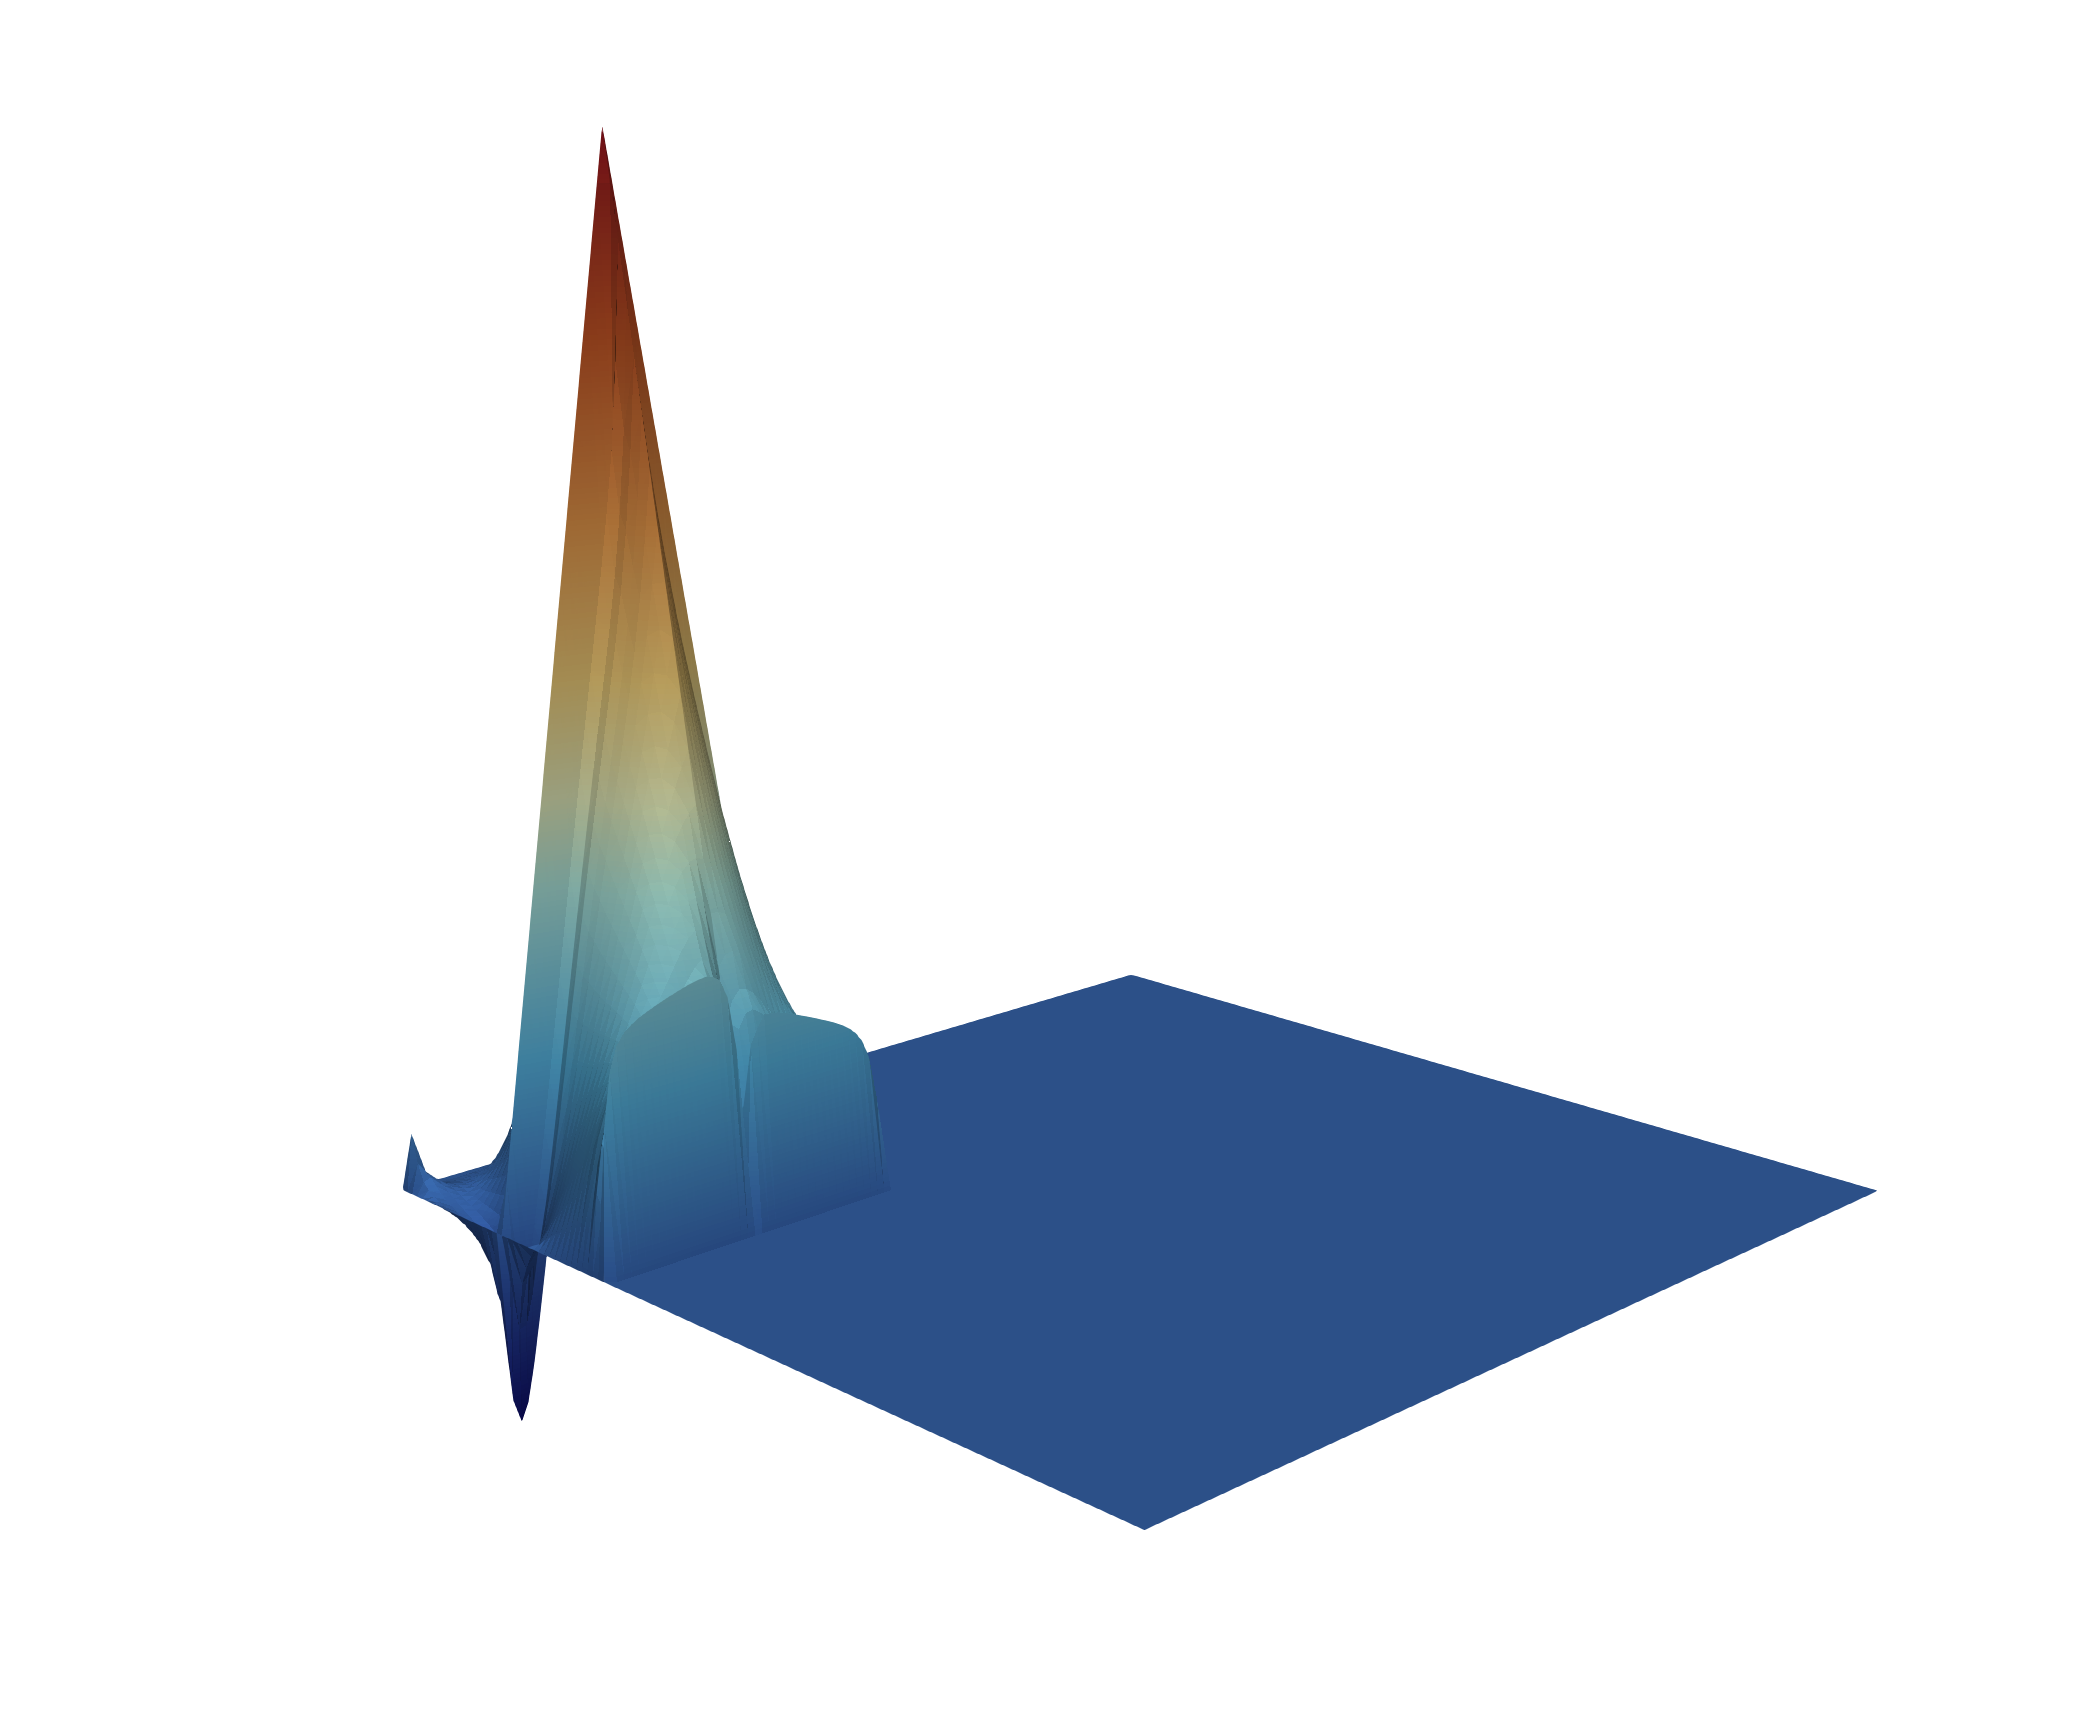
\includegraphics[width=\textwidth]{images/MsFEM-x}
			\caption{MsFEM $x$-component.}
		\end{subfigure}
		\caption{Components of $x$-velocity coarse basis function.}
	\end{figure}
\end{frame}

\begin{frame}{MsFEM vs. RGDSW, 256 subdomains}
	% Mention that: 
	%   - Re has no effect 
	%   - MsFEM was faster for Re=1000 but maybe RGDSW can be sped up with proper tuning
	%   - These results were generated with higher GMRES tollerance which increases GMRES count and runtime without a positive effect
	\begin{figure}
		\centering
		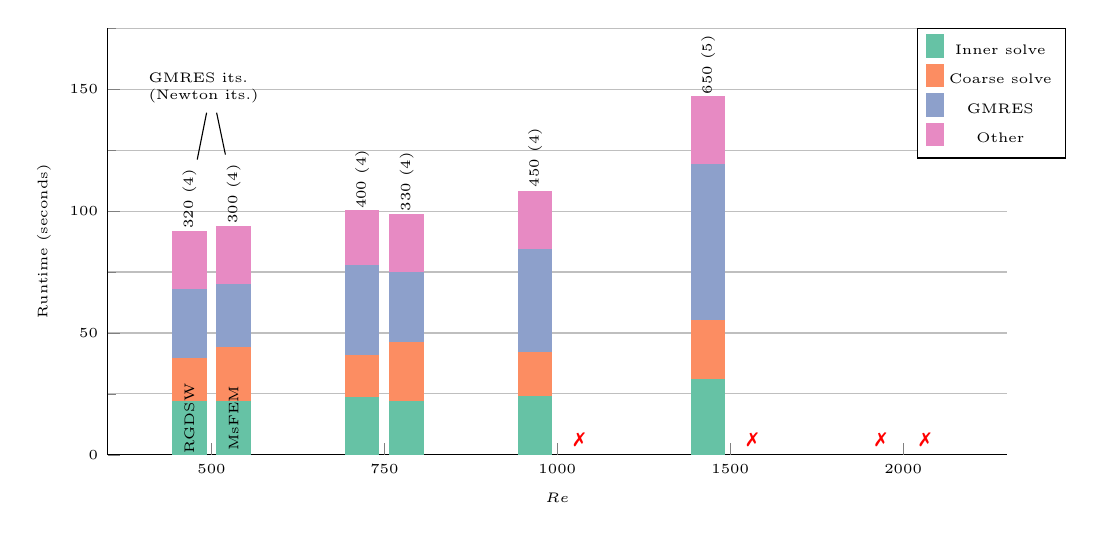
\begin{tikzpicture}
	\pgfplotsset{
		every axis/.append style={
				ybar stacked,
				width=13cm,
				height=7cm,
				ylabel={Runtime (seconds)},
				xlabel={$Re$},
				symbolic x coords={500, 750, 1000, 1500, 2000},
				xtick=data,
				enlarge x limits=0.15,
				legend style={at={(0.9,1)},anchor=north west},
				axis lines*=left, ymajorgrids, yminorgrids,
				ymin=0,
				ymax=175,
				bar width=12pt,
				minor y tick num=1,
				xticklabel style={rotate=0,xshift=0ex,anchor=north},
				cycle list name=Set2-5,
			},
		% Ensures that bars are plotted full
		every axis plot/.append style={
				fill,
			},
	}
	% RGDSW
	\begin{axis}[bar shift=-8pt, hide axis]
		\node [rotate=90](rgdsw) at ([xshift=-8pt]axis cs:500,15) {RGDSW};
		% Inner solve
		\addplot coordinates {(500,22) (750,23.7) (1000,23.8) (1500,31) (2000,0)};
		% Coarse solve
		\addplot coordinates {(500,17.4) (750,17.1) (1000,18.3) (1500,24) (2000,0)};
		% GMRES
		\addplot coordinates {(500,28.6) (750,37) (1000,42.2) (1500,64) (2000,0)};
		% Other
		\addplot coordinates {(500,23.7) (750,22.6) (1000,23.7) (1500,28) (2000,0)};

		\node [rotate=90,anchor=center](500) at ([xshift=-8pt]axis cs:500,105) {$320$ $(4)$};
		\node [rotate=90,anchor=center](750) at ([xshift=-8pt]axis cs:750,113) {$400$ $(4)$};
		\node [rotate=90,anchor=center](1000) at ([xshift=-8pt]axis cs:1000,122) {$450$ $(4)$};
		\node [rotate=90,anchor=center](1500) at ([xshift=-8pt]axis cs:1500,160) {$650$ $(5)$};
		\node at ([xshift=-8pt]axis cs:2000,6) {\scriptsize\color{red}\ding{55}};

	\end{axis}

	\begin{axis}[bar shift=8pt]
		\node [rotate=90](msfem) at ([xshift=8pt]axis cs:500,15) {MsFEM};
		% Inner solve
		\addplot coordinates {(500,21.9) (750,21.9) (1000,0) (1500,0) (2000,0)};
		% Coarse solve                            
		\addplot coordinates {(500,22.3) (750,24  ) (1000,0) (1500,0) (2000,0)};
		% GMRES                                   
		\addplot coordinates {(500,25.6) (750,28.9) (1000,0) (1500,0) (2000,0)};
		% Other                                   
		\addplot coordinates {(500,23.7) (750,23.9) (1000,0) (1500,0) (2000,0)};


		\legend{
			Inner solve,
			Coarse solve,
			GMRES,
			Other
		}
		\node[rotate=90,anchor=center](one) at ([xshift=8pt]axis cs:500,107) {$300$ $(4)$};
		\node[rotate=90,anchor=center] at ([xshift=8pt]axis cs:750,112) {$330$ $(4)$};

		\node at ([xshift=8pt]axis cs:1000,6) {\scriptsize\color{red}\ding{55}};
		\node at ([xshift=8pt]axis cs:1500,6) {\scriptsize\color{red}\ding{55}};
		\node at ([xshift=8pt]axis cs:2000,6) {\scriptsize\color{red}\ding{55}};


	\end{axis}

	\node[rotate=0, text width=1.6cm] (gmres) at ([xshift=8,yshift=40]500){GMRES its. (Newton its.)};
	% \node[rotate=0, text width=1.8cm] (coarsespace) at ([yshift=-60,xshift=-10]1000){Coarse space};

	\draw [thin] (gmres) --  (500);
	\draw [thin] (gmres) --  (one);

	% \draw [thin] (coarsespace) --  (rgdsw);
	% \draw [thin] (coarsespace) --  (msfem);

\end{tikzpicture}

		\label{fig:msfem-vs-rgdsw}
	\end{figure}
\end{frame}

\begin{frame}{Summary lid-driven cavity}
	\begin{itemize}
		\item Excellent weak scalability up to $9216$ subdomains. % (larger coarse space improves nonlinear preconditioning)
		\item Hybrid is more robust than NKS against nonlinearity.
		\item The two-level nonlinear Schwarz method is highly sensitive\\to variations in the coarse space.
		\item It's difficult to tune, e.g., what makes a good coarse space?%: many parameters that have a potentialy significant impact on performance
	\end{itemize}
	\vspace{2mm}
	\begin{center}
		\includegraphics[width=0.5\textwidth]{images/nls.png}\\
		{\tiny \vspace{-2mm}\hspace{-4.6cm}Generated with ChatGPT}
	\end{center}
	% Bottom line: very sensitive to proper tuning, The coarse space does not encode the Re somehow but it's discretisation properties are critical.
\end{frame}


\section{Outlook}
\begin{frame}{Outlook}
    \begin{itemize}
        \item Publish neo-Hookean and lid-driven cavity results
        \item Complete interface with FEAT3
        \item Run the following tests: 3D, non-Newtonian fluids, complex geometries
    \end{itemize}
    \vspace*{4mm}
    \only<2>{
        \begin{block}{Acknowledgments}
            \begin{itemize}
                \item Generous assistance from:
                  \begin{itemize}
                    \item {\bf Alexander Heinlein} (TU Delft) with FROSch implementation details
                    % \item {\bf Sharan Nurani Ramesh} (RUB) with the beam model
                    \item {\bf Lea Saßmannshausen} (UoC) with the FEDDLib
                  \end{itemize}
                \item Funded by the {\bf Bundesministerium für Forschung, Technologie und Raumfahrt} (BMFTR) through the project StroemungsRaum - Novel Exascale-Architectures with Heterogeneous Hardware Components for Computational Fluid Dynamics Simulations 
                \item Computations done on the NHR cluster Fritz
            \end{itemize}   
        \end{block}    
    }
\end{frame}



\begin{frame}[noframenumbering]{}
    \vspace*{6mm}
\begin{center}
    \huge Thanks for your attention!\\ Any questions?
\end{center}
\end{frame}

\begin{frame}[noframenumbering]{Nonlinear Laplace: solver settings}
	\begin{itemize}
		\item $300\times 300$ elements per subdomain
		\item Averaging recombination
		\item Relative tolerance outer Newton: $10^{-4}$
		\item GMRES tolerance: $10^{-6}$
		\item Relative tolerance inner Newton: $10^{-5}$
		\item Absolute tolerance inner Newton: $10^{-11}$
		\item RGDSW coarse space
		\item Zero initial value
	\end{itemize}
\end{frame}

\begin{frame}[noframenumbering]{Neo-Hooke: Solver settings}
	\begin{columns}
		\begin{column}{0.55\textwidth}
			General settings:
			\vspace{7pt}
			\begin{itemize}
				\item Outer Newton rel. tol.  = $10^{-4}$
				\item Outer Newton max. iters. = $10$
				\item GMRES rel. tol. = $10^{-6}$
				\item GMRES max. its. = $100$
				\item Recombination mode: averaging
				      % Note: overlap used here is the dual graph overlap. Actual overlap used for NKS = 5 to correspond to similar physicial overlap
				\item Coarse space: MsFEM elasticity with overlap = $5$
			\end{itemize}
		\end{column}%
		\begin{column}{0.45\textwidth}
			Nonlinear Schwarz specific settings:
			\vspace{7pt}
			\begin{itemize}
				\item Inner Newton rel. tol. = $10^{-3}$
				\item Inner Newton abs. tol. = $10^{-9}$
				\item Inner Newton max. iters. = $15$
				\item Dual graph overlap = $10$
			\end{itemize}
		\end{column}
	\end{columns}
\end{frame}

\begin{frame}[noframenumbering]{LDC: solver settings}
	\begin{columns}
		\begin{column}{0.55\textwidth}
			General settings:
			\vspace{7pt}
			\begin{itemize}
				\item Subdomain size: $150\times 150$ elements
				\item Outer Newton rel. tol.  = \num{e-6}
				\item Outer Newton abs. tol.  = \num{e-6}
				\item Backtracking line-search
				\item GMRES rel. tol. = \num{e-4}
				\item GMRES max. its. = $1000$
				\item Krylov subspace dim. = $500$
				\item Recombination mode: averaging
				\item Coarse space: RGDSW with overlap = $5$
			\end{itemize}
		\end{column}%
		\begin{column}{0.45\textwidth}
			Nonlinear Schwarz specific settings:
			\vspace{7pt}
			\begin{itemize}
				\item Inner Newton rel. tol. = \num{e-3}
				\item Inner Newton abs. tol. = \num{e-14}
				\item Inner Newton max. iters. = $50$
				\item Hybrid variant
			\end{itemize}
		\end{column}
	\end{columns}
\end{frame}

\begin{frame}[noframenumbering]{Adding a second level}
	Build coarse space basis functions $\rightarrow$ $R_0$ and $P_0$
	\begin{block}{RGDSW coarse space \footnotemark{}}
		Define coarse basis $\Phi : V_0\mapsto V$
		\begin{enumerate}
			\setlength{\itemsep}{10pt}
			\item Build $\Phi_\Gamma$ as a partition of unity on the interface $\Gamma$
			\item $\Phi_I = -A_{II}^{-1}A_{I\Gamma}\Phi_\Gamma$ an energy minimizing extension into the interior
		\end{enumerate}
	\end{block}
	\only<2>{ % Compile twice for proper placement
		For example:
		\begin{columns}
			\begin{column}{0.39\textwidth}
				\vspace*{-6mm}
				\begin{figure}
					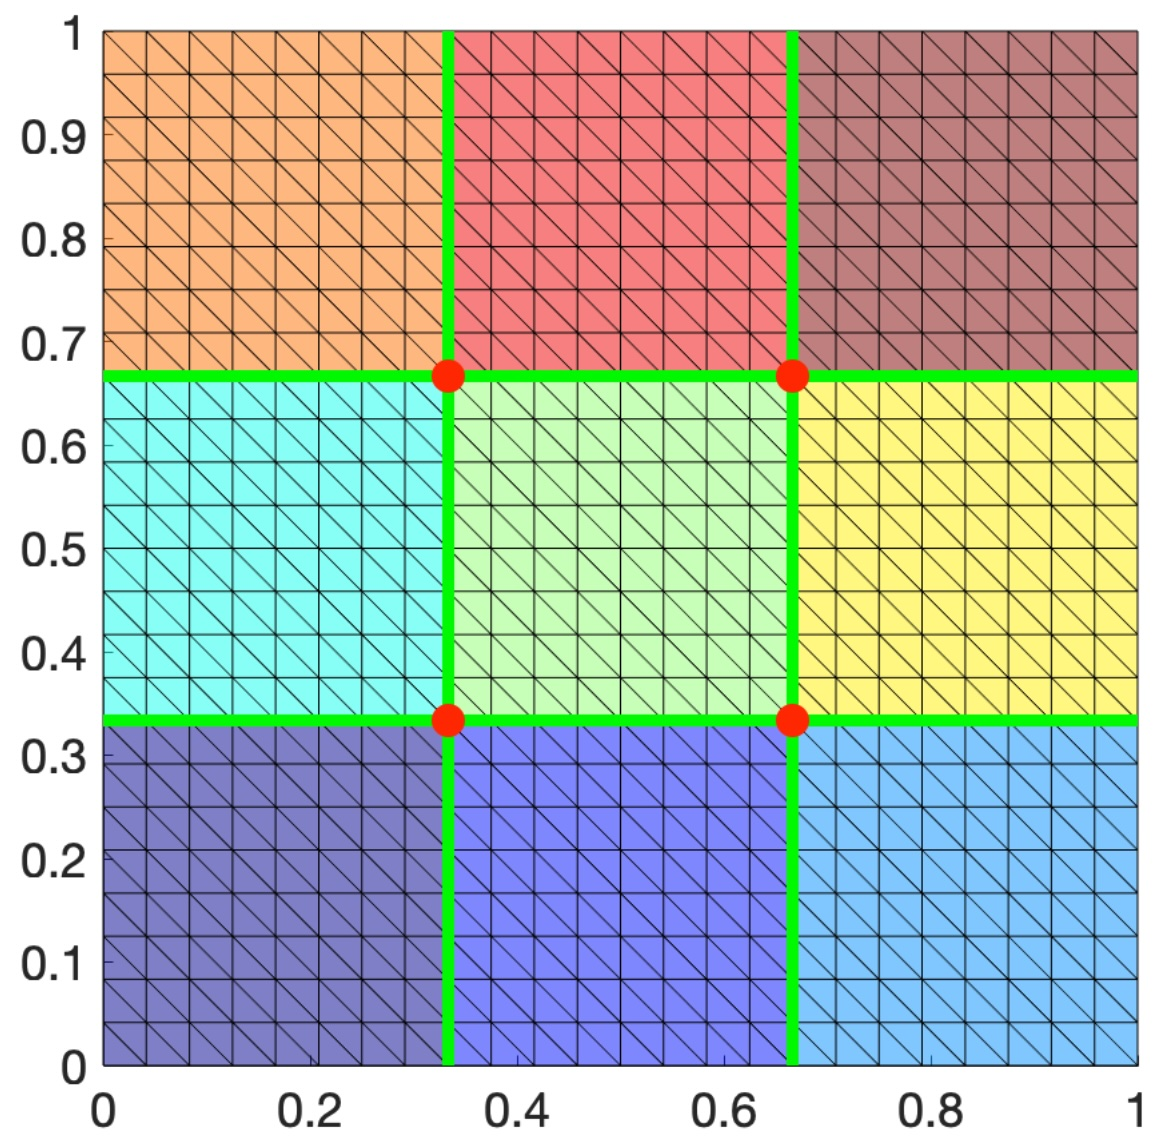
\includegraphics[width=0.45\textwidth]{images/decomposed_domain.jpg}
				\end{figure}
			\end{column}
			\hspace*{-20mm}
			\begin{column}{0.4\textwidth}
				\vspace*{-9mm}
				\begin{figure}
					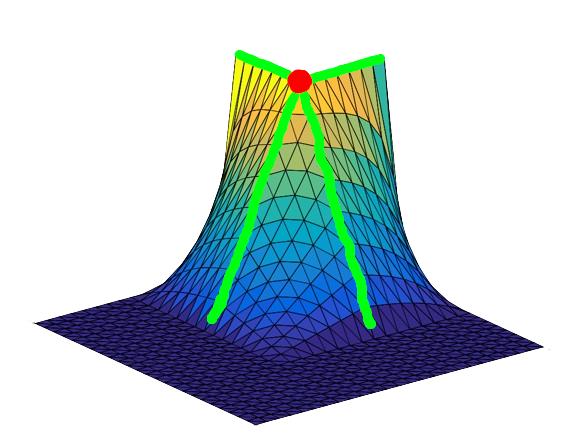
\includegraphics[width=0.65\textwidth]{images/r22.png}
				\end{figure}
			\end{column}
		\end{columns}
	}
	\only<3>{
		Summary:
		\begin{equation*}
			\Phi =
			\begin{pmatrix}
				\Phi_I \\  \Phi_\Gamma
			\end{pmatrix} =
			\begin{pmatrix}
				-A_{II}^{-1}A_{I\Gamma}\Phi_\Gamma \\ \Phi_\Gamma
			\end{pmatrix}
		\end{equation*}
		and
		\begin{equation*}
			P_0 \coloneqq \Phi\text{,}\quad R_0 \coloneqq \Phi^T
		\end{equation*}
	}
	\footnotetext{\tiny Dohrmann, Widlund (2017)}
\end{frame}

\begin{frame}[noframenumbering]{Motivation: linear vs nonlinear preconditioning}
	Discretized nonlinear partial differential equation: $F(u) = 0$
	\begin{columns}
		\begin{column}{0.5\textwidth}
			\vspace*{-4mm}
			\begin{block}{\normalsize Linear preconditioner}
				\begin{enumerate}
					\item Linearize:
					      \begin{equation*}
						      DF(u^k)\delta^{k+1} = F(u^k)
					      \end{equation*}
					\item Improve linear solver performance with Schwarz preconditioner:
					      \begin{equation*}
						      \mathcal{M}_{OS}^{-1}DF(u^k)\delta^{k+1} = \mathcal{M}_{OS}^{-1}F(u^k)
					      \end{equation*}
				\end{enumerate}
				\vspace*{4mm}
				Goal:
				\begin{itemize}
					\item $\kappa(\mathcal{M}_{OS}^{-1}DF(u^k)) \approx 1$
				\end{itemize}
			\end{block}
		\end{column}
		\begin{column}{0.5\textwidth}
			\vspace*{-4mm}
			\begin{block}{\normalsize Nonlinear preconditioner}
				\begin{enumerate}
					\item Reformulate the original nonlinear problem based on local nonlinear corrections
					      \begin{equation}
						      \mathcal{F}(u) = G(F(u)) = 0
					      \end{equation}
					\item Linearize $\mathcal{F}(u) = 0$ and solve iterativily
				\end{enumerate}
				Goal:
				\begin{itemize}
					\item $\mathcal{F}(u)$ more linear than $F(u)$
					\item $\mathcal{F}(u^*) = 0 \iff F(u^*) = 0$
				\end{itemize}
			\end{block}
		\end{column}
	\end{columns}

\end{frame}

\begin{frame}[noframenumbering]{One-level nonlinear Schwarz}
	\note{This requires two levels of Newton's method. Seems to be less efficient at first glance. The advantage of this method becomes apparent when solving problems with local regions of highly nonlinear behavior e.g. laminar flow with localized turbulence\\}
	\note{The algorithm shows how this method is essentially the same as applying Newton directly, but to the function $\mathcal{F}$ instead of $F$.\\}
	\note{Constructin $A$ requires inversion of all the local matrices. The result of this is that the linear system is already preconditioned. Note that the preconditioner can not be changed on the fly. It results directly from the nonlinear problem}
	\begin{columns}
		\begin{column}{0.53\textwidth}
			\begin{algorithm}[H]
				\small
				\begin{algorithmic}[1]
					\State $k\gets0$
					\State \textbf{Init.} $u^k$
					\State \textbf{Eval.} $F(u^k)$
					\While{stop. cond. false}
					\State \textbf{Eval.} $\mathcal{F}_1(u^k)$
					\State \textbf{Eval.} $D\mathcal{F}_1(u^k)$
					\State \textbf{Solve} (e.g. GMRES) $D\mathcal{F}_1(u^k)\delta^k = \mathcal{F}_1(u^k)$
					\State \textbf{Update} $u^{k+1} = u^k - \delta^k$
					\State $k\gets k+1$
					\State \textbf{Eval.} $F(u^k)$
					\EndWhile
				\end{algorithmic}
				\caption*{\small Nonlinear Schwarz}
			\end{algorithm}
		\end{column}
		\begin{column}{0.47\textwidth}
			\begin{algorithm}[H]
				\small
				\begin{algorithmic}[1]
					\State $k \gets 0$
					\State \textbf{Init.} $g_i^k$
					\State \textbf{Eval.} $F_i^k\coloneqq R_iF(u-P_ig_i^k)$
					\While{stop. cond. false}
					\State \textbf{Eval.} $DF_i^k= R_iDF(u-P_ig_i^k)P_i$
					\State \textbf{Solve} (direct) $DF_i^k\delta^k = F_i^k$
					\State \textbf{Update} $g_i^{k+1} = g_i^k + \delta^k$
					\State $k\gets k+1$
					\State \textbf{Eval.} $F_i^k\coloneqq R_iF(u-P_ig_i^k)$
					\EndWhile
					\State $g_i\gets g_i^k$
				\end{algorithmic}
				\caption*{\small Evaluation of $g_i\coloneqq T_i(u)$}
			\end{algorithm}
		\end{column}
	\end{columns}
\end{frame}

\begin{frame}[noframenumbering]{Nonlinear Schwarz domain decomposition methods}% \footnote{\tiny Cai and Keyes 2002} \footnote{\tiny Dolean, Gander, Cherie, Kwok and Masson 2016}}
	\vspace{-5mm}
	\begin{columns}
		\begin{column}{0.7\textwidth}
			\centering
			\begin{block}{\normalsize Alternative nonlinear problem}
				The discretized nonlinear partial differential equation
				\begin{equation*}
					F(u) = 0,\, F : V\mapsto V
				\end{equation*}
				is reformulated to
				\begin{equation*}
					\mathcal{F}(u) = 0,\, \mathcal{F} : V\mapsto V.
				\end{equation*}
				The new nonlinear function $\mathcal{F}(u)$ is given implicitly by computing local nonlinear corrections $T_i(u),\,i = 1,\dots,N$ on (overlapping) subdomains
			\end{block}
		\end{column}
		\begin{column}{0.3\textwidth}
			\begin{figure}
				
\includegraphics[height=0.4\textwidth,width=0.7\textwidth]{images/DD-mesh-1.png}
				\vspace{-2mm}
				\caption{\tiny Global domain $\Omega$, FE space $V$}
			\end{figure}
			\vspace{-6mm}
			\begin{figure}
				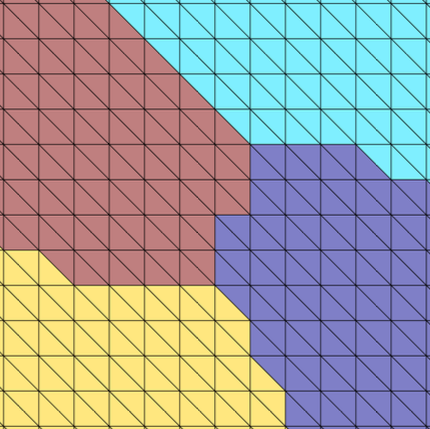
\includegraphics[height=0.4\textwidth,width=0.7\textwidth]{images/DD-mesh-2.png}
				\vspace{-2mm}
				\caption{\tiny Subdomains $\Omega_i$, FE spaces $V(\Omega_i)$}
			\end{figure}
			\vspace{-6mm}
			\begin{figure}
				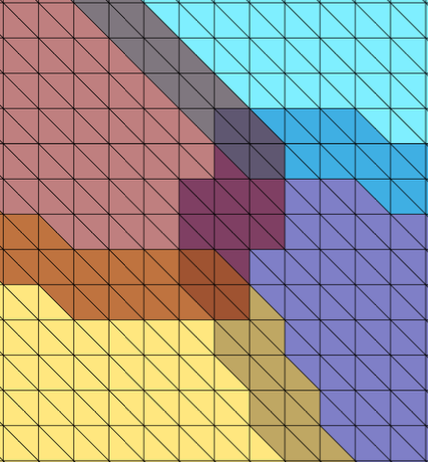
\includegraphics[height=0.4\textwidth,width=0.7\textwidth]{images/DD-mesh-3.png}
				\vspace{-2mm}
				\caption{\tiny Overlapping SDs $\Omega_i'$, FE spaces $V_i$}
			\end{figure}
		\end{column}

	\end{columns}
\end{frame}

\begin{frame}[noframenumbering]{Adding a coarse level \footnote{\tiny Toselli, Widlund (2005)}}

	{\Large Linear Schwarz preconditioners}
	\vspace*{4mm}
	\begin{columns}
		\begin{column}{0.5\textwidth}
			{\bf One-level Schwarz preconditioner}
			\begin{equation*}
				\mathcal{M}^{-1}_{OS-1}=\sum_{i=1}^{N}P_i(R_iAP_i)^{-1}R_i
			\end{equation*}
			\begin{block}{\normalsize Condition number estimate:}
				\begin{equation*}
					\kappa(\mathcal{M}^{-1}_{OS-1}A)\leq C(1+\frac{1}{H\delta})
				\end{equation*}
			\end{block}
		\end{column}
		\begin{column}{0.5\textwidth}
			{\bf Two-level Schwarz preconditioner}
			\vspace*{3mm}
			\begin{equation*}
				\mathcal{M}^{-1}_{OS-2}=P_0(R_0AP_0)^{-1}R_0 + \mathcal{M}^{-1}_{OS-1}
			\end{equation*}
			\begin{block}{\normalsize Condition number estimate:}
				\begin{equation*}
					\kappa(\mathcal{M}^{-1}_{OS-2}A)\leq C(1+\frac{H}{\delta})
				\end{equation*}
			\end{block}
		\end{column}
	\end{columns}
	\vspace*{4mm}
	\centering
	with subdomain size $H$ and overlap width $\delta$
	% \let\thefootnote\relax\footnote{Dohrmann, Widlund 2012}
\end{frame}

\begin{frame}[noframenumbering]{Hyperelasticity coarse basis modification}
	\centering
	\vspace{10mm}
	\only<1>{
		\begin{tikzpicture}
	\node[anchor=north west] (main) at (0, 0) {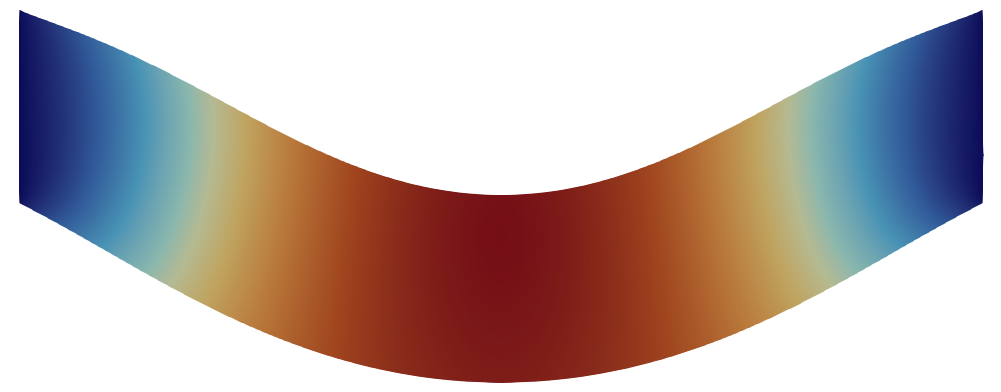
\includegraphics[width=0.65\textwidth]{images/beam-entire.png}};
	\node[anchor=south west,outer sep=0pt] (zoom) at (10.5, -3) {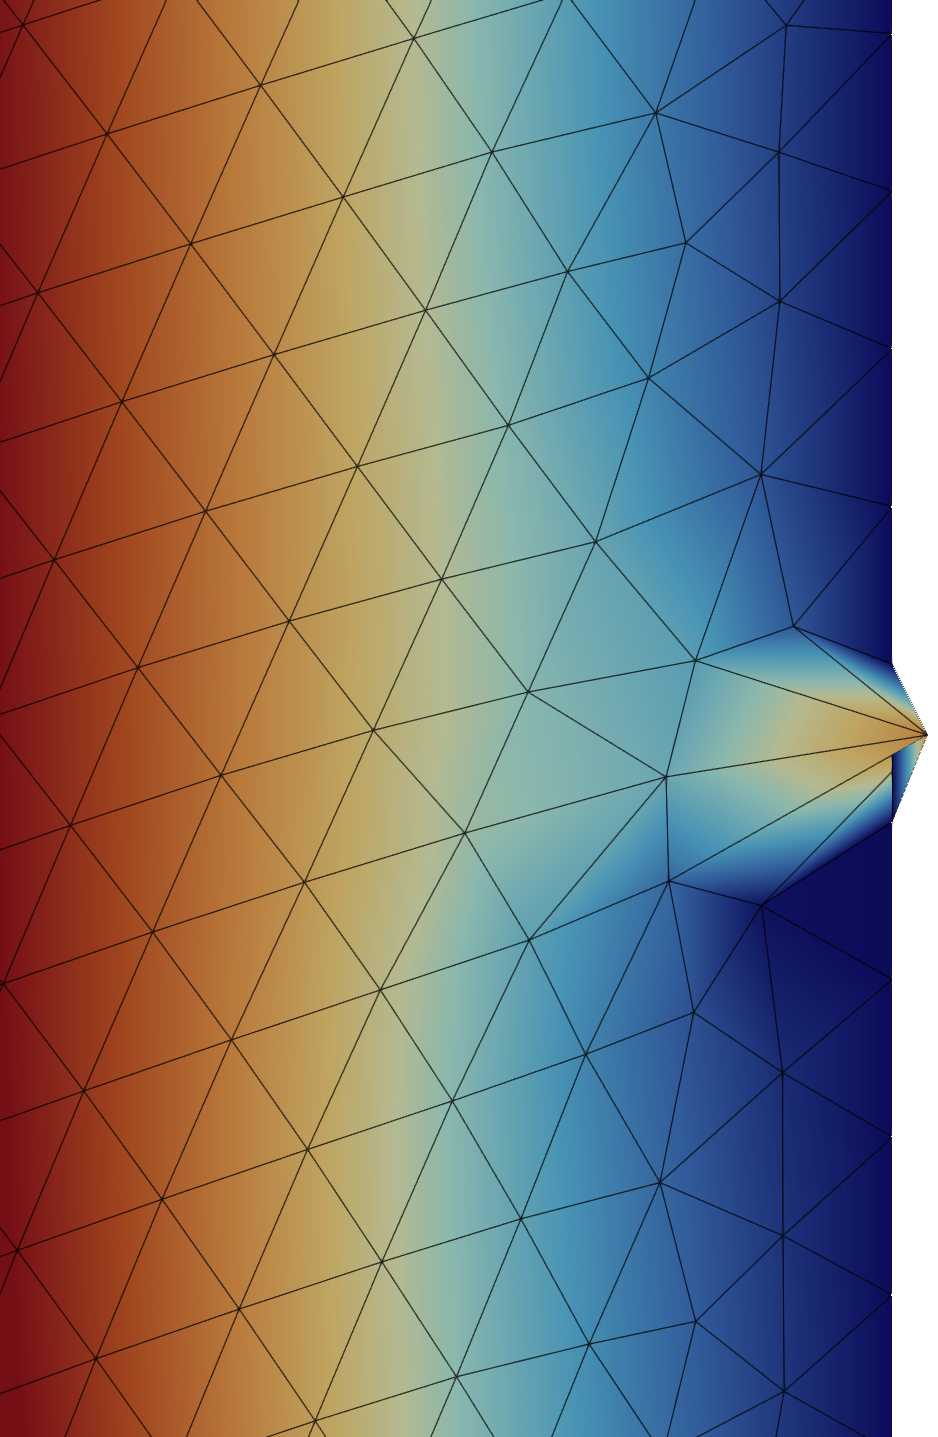
\includegraphics[width=0.15\textwidth]{images/beam-instability.png}};
	\node [draw, thick, minimum size=5mm,outer sep=0pt,red] (a) at ([xshift=-4mm,yshift=4mm]main.east){};

	\draw [thick, dashed] (a.north east) -- ([yshift=-2mm]zoom.north west);
	\draw [thick, dashed] (a.south east) -- ([yshift=2mm]zoom.south west);
\end{tikzpicture}

	}
	\only<2>{
		\begin{tikzpicture}
	\node[anchor=north west] (main) at (0, 0) {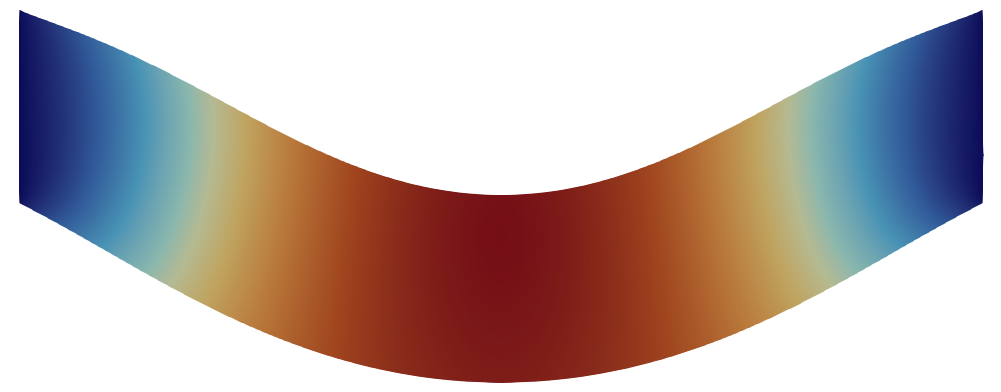
\includegraphics[width=0.65\textwidth]{images/beam-entire.png}};
	\node[anchor=south west,outer sep=0pt] (zoom) at (10.5, -3) {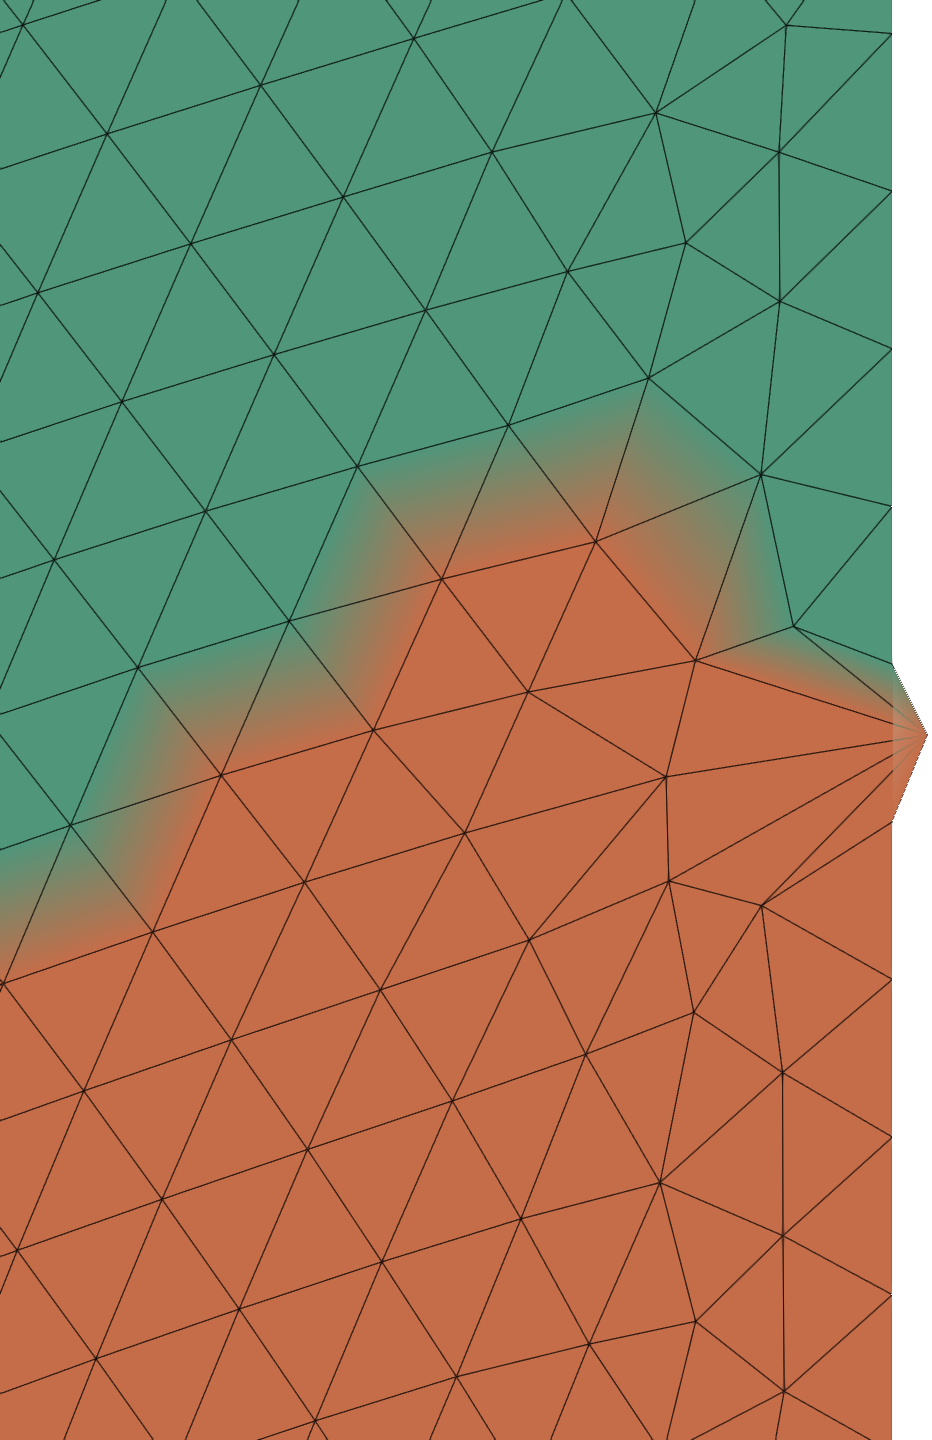
\includegraphics[width=0.15\textwidth]{images/beam-instability-boundary.png}};
	\node [draw, thick, minimum size=5mm,outer sep=0pt,red] (a) at ([xshift=-4mm,yshift=4mm]main.east){};

	\draw [thick, dashed] (a.north east) -- ([yshift=-2mm]zoom.north west);
	\draw [thick, dashed] (a.south east) -- ([yshift=2mm]zoom.south west);
\end{tikzpicture}

	}
\end{frame}

\begin{frame}[noframenumbering]{Hyperelasticity coarse basis modification}
	\begin{figure}[h!]
		\begin{subfigure}{0.49\textwidth}
			\centering
			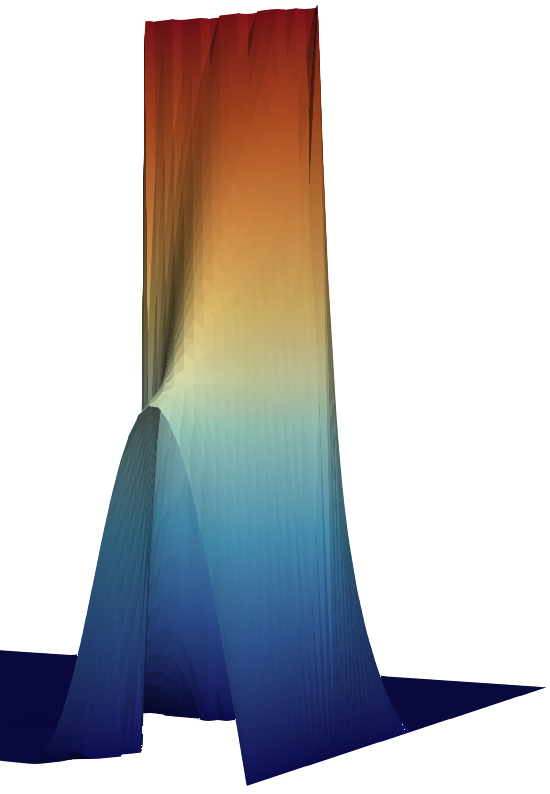
\includegraphics[width=0.7\textwidth,height=0.33\textheight]{images/beam-coarse-basis-1.png}
			\caption{\hspace{-20mm}Side view original}
		\end{subfigure}
		\hfill
		\begin{subfigure}{0.49\textwidth}
			\centering
			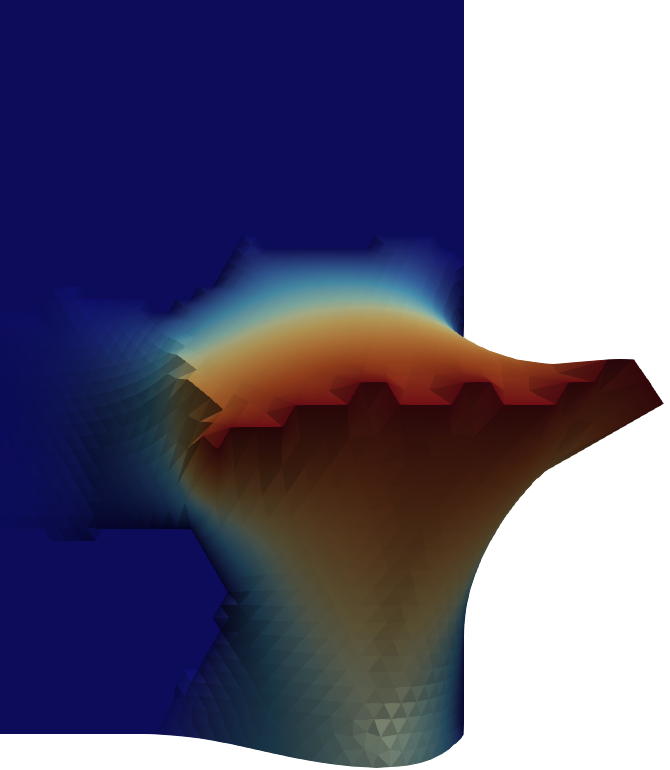
\includegraphics[width=0.7\textwidth,height=0.33\textheight]{images/beam-coarse-basis-2.png}
			\caption{\hspace{-20mm}Top view original}
		\end{subfigure}
		\vfill
		\visible<2->{
			\begin{subfigure}{0.49\textwidth}
				\centering
				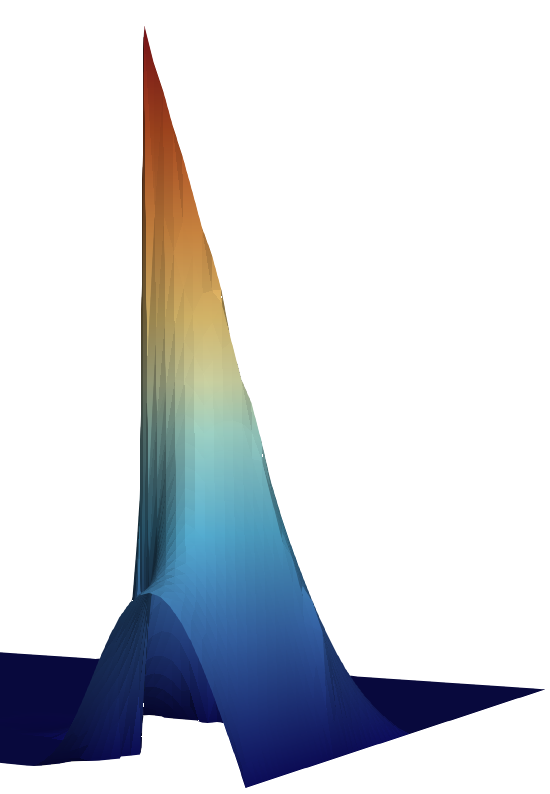
\includegraphics[width=0.7\textwidth,height=0.33\textheight]{images/beam-coarse-basis-3.png}
				\caption{\hspace{-20mm}Side view modified}
			\end{subfigure}
			\hfill
			\begin{subfigure}{0.49\textwidth}
				\centering
				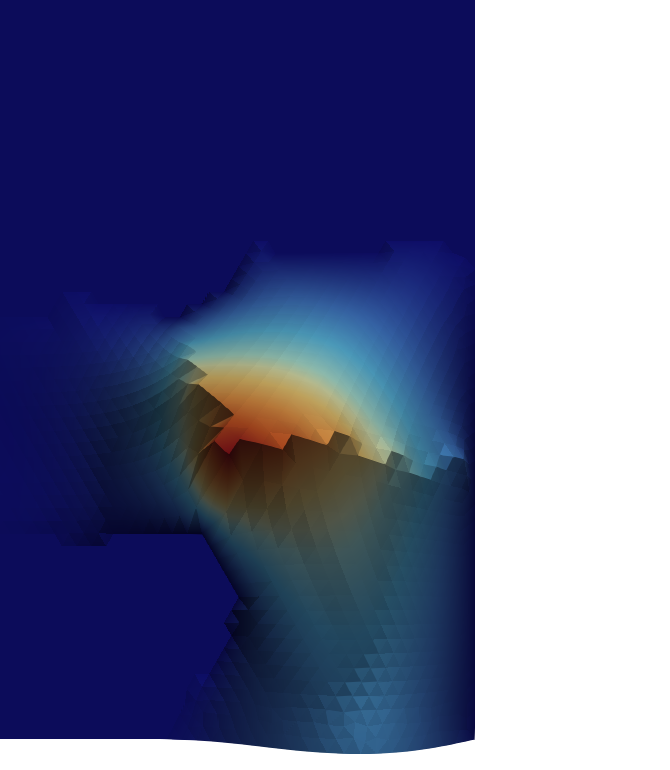
\includegraphics[width=0.7\textwidth,height=0.33\textheight]{images/beam-coarse-basis-4.png}
				\caption{\hspace{-20mm}Top view modified}
			\end{subfigure}
		}
	\end{figure}
\end{frame}



\begin{frame}[noframenumbering]{Sanity check: nonlinear Laplace}
	\begin{columns}
		\begin{column}{0.47\textwidth}
			\begin{align*}
				-\nabla\cdot((u^2+1)\nabla u) & =1\quad \text{in}\quad \Omega\subset\mathbb{R}^2, \\
				u                             & = 0\quad\text{on}\quad\partial\Omega              \\
				u^0                           & = 0
			\end{align*}
			\begin{figure}
				\centering
				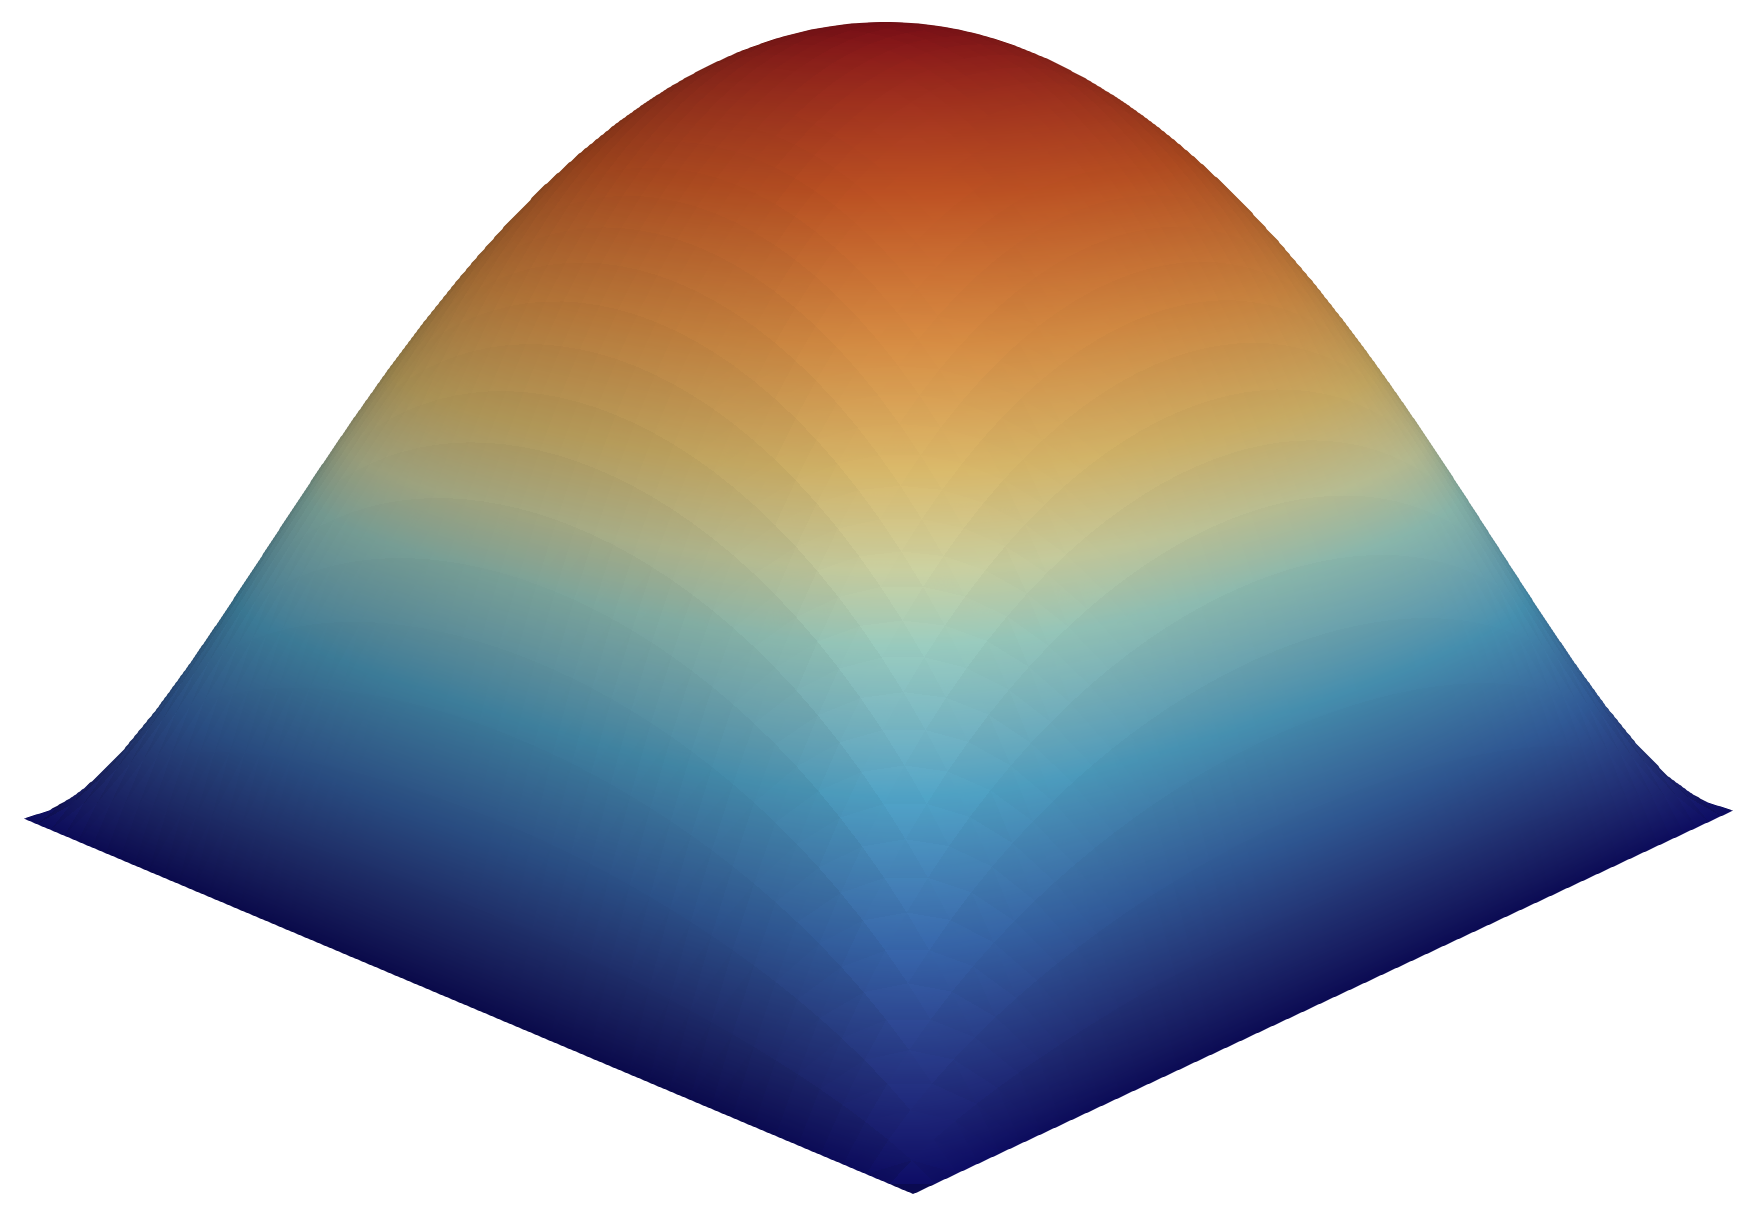
\includegraphics[width=0.45\textwidth]{images/laplace}
			\end{figure}
		\end{column}
		\begin{column}{0.53\textwidth}
			\begin{itemize}
				\setlength{\itemsep}{10pt}
				\item Subdomain size: $300\times300$ elements
				\item Solver relative tolerance: $10^{-4}$
				\item MsFEM coarse space
			\end{itemize}
		\end{column}
	\end{columns}
\end{frame}

\begin{frame}[noframenumbering]{Sanity check: weak scalability}
	\begin{figure}
		\centering
		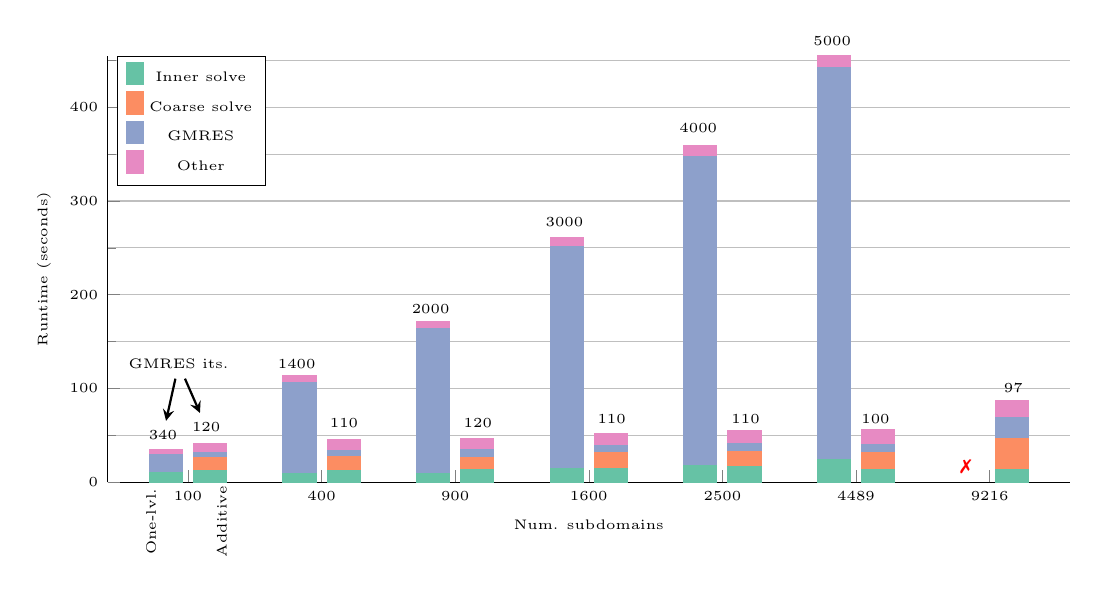
\begin{tikzpicture}
    \pgfplotsset{
      every axis/.append style={
    legend style={at={(0.01,1)},anchor=north west},
    axis lines*=left, ymajorgrids, yminorgrids,
    width=13.8cm, height=7cm,
    ymin=0,
    ymax=455,
    ybar stacked,
    bar width=12pt,
    minor y tick num=1,
    xtick={1,2,3,4,5,6,7},
    % xticklabels={100, 400, 900, 1600, 2500, 3600},
    %xmajorticks=false,
    xticklabels from table={\datatableonelevel}{SubdomainCount},
    xticklabel style={rotate=0,xshift=0ex,anchor=north},
    ylabel={Runtime (seconds)},
    xlabel={Num. subdomains},
      cycle list name=Set2-5,
    },
		every axis plot/.append style={
      fill,
    },
}
\pgfplotstableread{
Location SubdomainCount  GlobalSolve   InnerSolve   CoarseSolve   GMRES   Other
1        100             41.8	         12.6         13.55         5.8     9.85  
2        400	           45.5          12.94        14.0          7.1     11.46 
3        900             47.0          13.15        13.0          8.4     12.45 
4        1600            52.4          14.8         16.65         7.9     13.05 
5        2500            55.1          17.26        15.9          8.2     13.74 
% 6        3600            48.2          13.8         15.12         7.5     11.78 
6        4489            56.02         14           17.4          8.5     16.12 
7        9216            87            14           32.7          22      18.3 
}\datatabletwolevel
\pgfplotstableread{
Location SubdomainCount  GlobalSolve   InnerSolve   CoarseSolve   GMRES    Other
1        100             35.4          10.74        0             18.5     6.16  
2        400             113.6         9.6          0             96.9     7.1   
3        900             171.8         9.7          0             154.7    7.4   
4        1600	           261.2	       14.7		      0             236.3    10.2  
5        2500	           359.4	       18.24        0             328.7    12.46 
% 6        3600	           452.1	       20.9		      0             418.0    13.2  
6        4489            459           24           0             418      17    
7        9216            0             0            0             0        0 
}\datatableonelevel

\begin{axis}[bar shift=-8pt, hide axis]
    \addplot+ table [x=Location, y=InnerSolve] {\datatableonelevel};
    \addplot+ table [x=Location, y=CoarseSolve] {\datatableonelevel};
    \addplot+ table [x=Location, y=GMRES] {\datatableonelevel};
    \addplot+ table [x=Location, y=Other] {\datatableonelevel};
\end{axis}

\begin{axis}[bar shift=8pt]
    \addplot+ table [y=InnerSolve] {\datatabletwolevel}; \addlegendentry{Inner solve}
    \addplot+ table [y=CoarseSolve] {\datatabletwolevel}; \addlegendentry{Coarse solve}
    \addplot+ table [y=GMRES] {\datatabletwolevel}; \addlegendentry{GMRES}
    \addplot+ table [y=Other] {\datatabletwolevel}; \addlegendentry{Other}
\end{axis}
                            
\node[rotate=0] (gmres) at (0.9,1.5) {GMRES its.};
	
\node[rotate=0] (one) at (.7,0.6) {$340$};
\node[rotate=0] (two) at (1.25,0.7) {$120$};

\node[rotate=0] at (2.4,1.5) {$1400$};
\node[rotate=0] at (3.,.75) {$110$};

\node[rotate=0] at (4.1,2.2) {$2000$};
\node[rotate=0] at (4.7,0.75) {$120$};

\node[rotate=0] at (5.8,3.3) {$3000$};
\node[rotate=0] at (6.4,0.8) {$110$};

\node[rotate=0] at (7.5,4.5) {$4000$};
\node[rotate=0] at (8.1,0.8) {$110$};

\node[rotate=0] at (9.2,5.6) {$5000$};
\node[rotate=0] at (9.75,0.8) {$100$};

\node[rotate=0] at (10.9,.2) {\scriptsize\color{red}\ding{55}};
\node[rotate=0] at (11.5,1.2) {$97$};

\draw [arrow] (gmres) --  (one);
\draw [arrow] (gmres) --  (two);


\node[rotate=90] at (0.55,-0.5) {One-lvl.};
\node[rotate=90] at (1.45,-0.5) {Additive};

\end{tikzpicture}


















	\end{figure}
\end{frame}

\begin{frame}[noframenumbering]{StroemungsRaum consortium}
	% \hspace*{-2cm}
	% \vspace*{-1cm}
	\begin{figure}
		\centering
		\scalebox{0.8}{ % Adjust scale if needed
	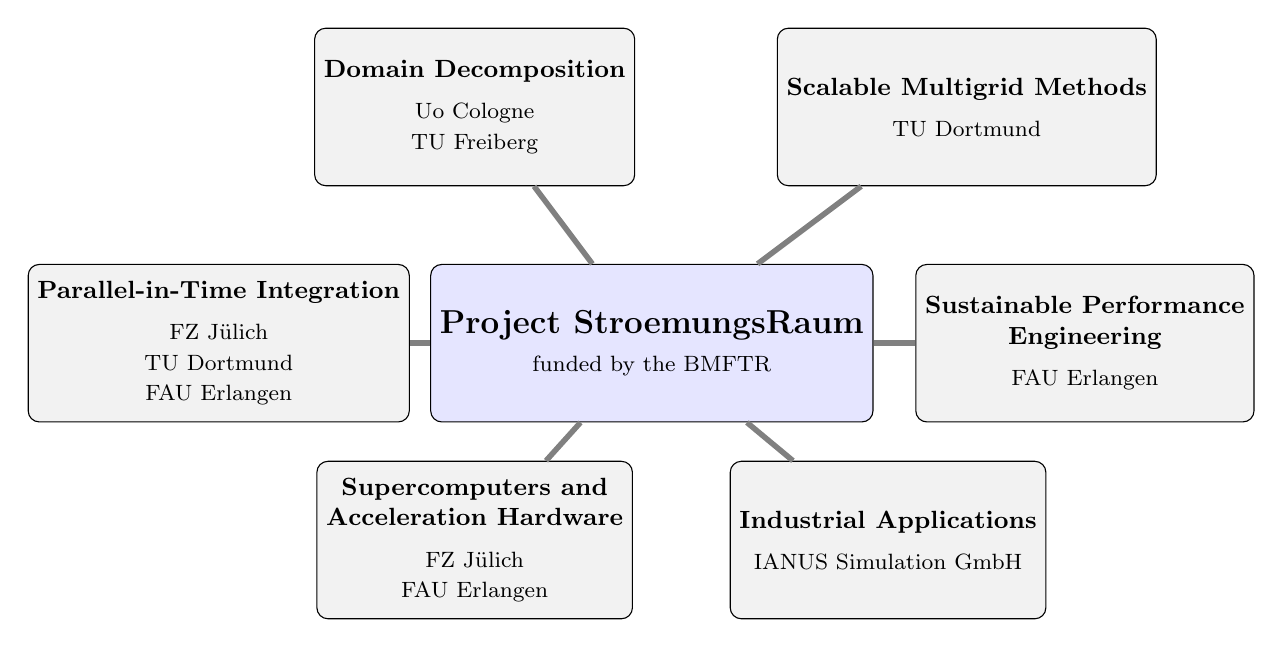
\begin{tikzpicture}[
			% Removed "mindmap" as it applies specific styling that's hard to override
			every node/.style={
					rectangle,
					rounded corners,
					minimum width=2cm,
					minimum height=2cm,
					align=center,
					font=\small,
					text=black,
					draw=black,
					fill=gray!10
				},
			root concept/.style={
					fill=blue!10,
					font=\bfseries\large,
					text=black,
					minimum width=3cm
				},
			% Custom edge style
			conn/.style={
					draw=black!50,
					line width=2pt,
					solid
				},
		]
		\begin{scope}[shift={(-5, 3)}]
			\node[root concept] (root) {Project StroemungsRaum\\{\normalfont\footnotesize funded by the BMFTR}};

			% Create child nodes with explicit positioning and manual edges
			\node[xshift=5.5cm, yshift=0cm] (n1) {\bf{Sustainable Performance}\\\bf{Engineering}\\[1ex]\footnotesize FAU Erlangen};
			\node[xshift=4cm, yshift=3cm] (n2) {\bf{Scalable Multigrid Methods}\\[1ex] \footnotesize TU Dortmund};
			\node[xshift=-2.25cm, yshift=3cm] (n3) {\bf{Domain Decomposition}\\[1ex]\footnotesize \alert{Uo Cologne}\\ \footnotesize TU Freiberg};
			\node[xshift=-5.5cm, yshift=0cm] (n4) {\bf{Parallel-in-Time Integration}\\[1ex] \footnotesize FZ Jülich\\ \footnotesize TU Dortmund\\ \footnotesize FAU Erlangen};
			\node[xshift=-2.25cm, yshift=-2.5cm] (n5) {\bf{Supercomputers and}\\\bf{Acceleration Hardware}\\[1ex] \footnotesize FZ Jülich\\\footnotesize FAU Erlangen};
			\node[xshift=3cm, yshift=-2.5cm] (n6) {\bf{Industrial Applications}\\[1ex] \footnotesize IANUS Simulation GmbH};
			%
			% % Draw thin connections
			\draw[conn] (root) -- (n1);
			\draw[conn] (root) -- (n2);
			\draw[conn] (root) -- (n3);
			\draw[conn] (root) -- (n4);
			\draw[conn] (root) -- (n5);
			\draw[conn] (root) -- (n6);
		\end{scope}
        % \node [inner sep=0pt] at (2,-0.5) {Project Stroemungsraum \includegraphics[width=0.25\textwidth]{images/StroemungsRaumMap.png}};
	\end{tikzpicture}
}

	\end{figure}
\end{frame}

\begin{frame}[noframenumbering]{Nonlinear preconditioning using FROSch}
	\begin{columns}
		\begin{column}{0.49\textwidth}
			\begin{block}{Two-level nonlinear Schwarz}
				\begin{itemize}
					\item Short info about nonlinear Schwarz
				\end{itemize}
			\end{block}
		\end{column}
		\begin{column}{0.49\textwidth}
			\begin{figure}
                \begin{subfigure}{\textwidth}
					\centering
					% 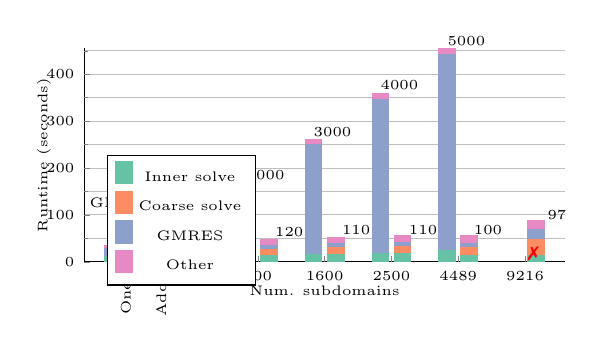
\begin{tikzpicture}[scale=0.5]
    \pgfplotsset{
      every axis/.append style={
    legend style={at={(0.01,1)},anchor=north west},
    axis lines*=left, ymajorgrids, yminorgrids,
    width=13.8cm, height=7cm,
    ymin=0,
    ymax=455,
    ybar stacked,
    bar width=12pt,
    minor y tick num=1,
    xtick={1,2,3,4,5,6,7},
    % xticklabels={100, 400, 900, 1600, 2500, 3600},
    %xmajorticks=false,
    xticklabels from table={\datatableonelevel}{SubdomainCount},
    xticklabel style={rotate=0,xshift=0ex,anchor=north},
    ylabel={Runtime (seconds)},
    xlabel={Num. subdomains},
      cycle list name=Set2-5,
    },
		every axis plot/.append style={
      fill,
    },
}
\pgfplotstableread{
Location SubdomainCount  GlobalSolve   InnerSolve   CoarseSolve   GMRES   Other
1        100             41.8	         12.6         13.55         5.8     9.85  
2        400	           45.5          12.94        14.0          7.1     11.46 
3        900             47.0          13.15        13.0          8.4     12.45 
4        1600            52.4          14.8         16.65         7.9     13.05 
5        2500            55.1          17.26        15.9          8.2     13.74 
% 6        3600            48.2          13.8         15.12         7.5     11.78 
6        4489            56.02         14           17.4          8.5     16.12 
7        9216            87            14           32.7          22      18.3 
}\datatabletwolevel
\pgfplotstableread{
Location SubdomainCount  GlobalSolve   InnerSolve   CoarseSolve   GMRES    Other
1        100             35.4          10.74        0             18.5     6.16  
2        400             113.6         9.6          0             96.9     7.1   
3        900             171.8         9.7          0             154.7    7.4   
4        1600	           261.2	       14.7		      0             236.3    10.2  
5        2500	           359.4	       18.24        0             328.7    12.46 
% 6        3600	           452.1	       20.9		      0             418.0    13.2  
6        4489            459           24           0             418      17    
7        9216            0             0            0             0        0 
}\datatableonelevel

\begin{axis}[bar shift=-8pt, hide axis]
    \addplot+ table [x=Location, y=InnerSolve] {\datatableonelevel};
    \addplot+ table [x=Location, y=CoarseSolve] {\datatableonelevel};
    \addplot+ table [x=Location, y=GMRES] {\datatableonelevel};
    \addplot+ table [x=Location, y=Other] {\datatableonelevel};
\end{axis}

\begin{axis}[bar shift=8pt]
    \addplot+ table [y=InnerSolve] {\datatabletwolevel}; \addlegendentry{Inner solve}
    \addplot+ table [y=CoarseSolve] {\datatabletwolevel}; \addlegendentry{Coarse solve}
    \addplot+ table [y=GMRES] {\datatabletwolevel}; \addlegendentry{GMRES}
    \addplot+ table [y=Other] {\datatabletwolevel}; \addlegendentry{Other}
\end{axis}
                            
\node[rotate=0] (gmres) at (0.9,1.5) {GMRES its.};
	
\node[rotate=0] (one) at (.7,0.6) {$340$};
\node[rotate=0] (two) at (1.25,0.7) {$120$};

\node[rotate=0] at (2.4,1.5) {$1400$};
\node[rotate=0] at (3.,.75) {$110$};

\node[rotate=0] at (4.1,2.2) {$2000$};
\node[rotate=0] at (4.7,0.75) {$120$};

\node[rotate=0] at (5.8,3.3) {$3000$};
\node[rotate=0] at (6.4,0.8) {$110$};

\node[rotate=0] at (7.5,4.5) {$4000$};
\node[rotate=0] at (8.1,0.8) {$110$};

\node[rotate=0] at (9.2,5.6) {$5000$};
\node[rotate=0] at (9.75,0.8) {$100$};

\node[rotate=0] at (10.9,.2) {\scriptsize\color{red}\ding{55}};
\node[rotate=0] at (11.5,1.2) {$97$};

\draw [arrow] (gmres) --  (one);
\draw [arrow] (gmres) --  (two);


\node[rotate=90] at (0.55,-0.5) {One-lvl.};
\node[rotate=90] at (1.45,-0.5) {Additive};

\end{tikzpicture}


















                    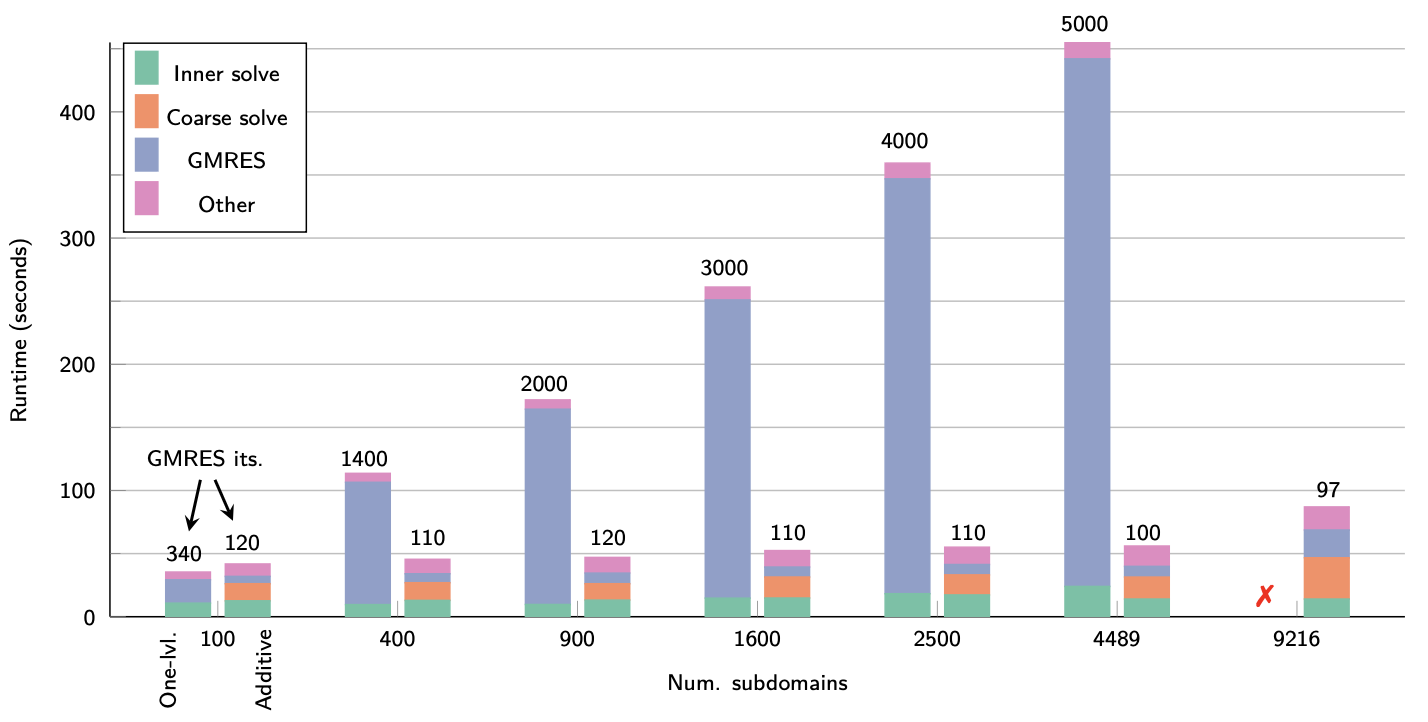
\includegraphics[width=\textwidth]{images/nonlin-laplace-scalability.png}
                    \caption{Weak scalability nonlinear diffusion}
				\end{subfigure}
                % \vspace{1mm}
                % \begin{subfigure}{0.4\textwidth}
                %     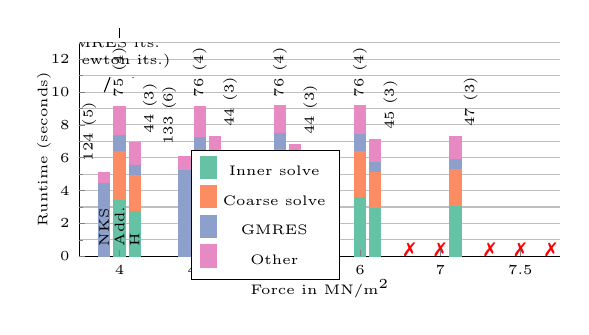
\begin{tikzpicture}[scale=0.5]
	\pgfplotsset{
		every axis/.append style={
				legend style={at={(1,1)},anchor=north east},
				axis lines*=left, ymajorgrids, yminorgrids,
				width=13.8cm, height=7cm,
				ymin=0,
				ymax=13,
				ybar stacked,
				bar width=8pt,
				minor y tick num=1,
				symbolic x coords={1,2,3,4,5,6},
				xtick={1,2,3,4,5,6},
				xticklabels from table={\hybrid}{Force},
				xticklabel style={rotate=0,xshift=0ex,anchor=north},
				ylabel={Runtime (seconds)},
				xlabel={Force in MN/m$^{2}$},
				cycle list name=Set2-5,
			},
		every axis plot/.append style={fill},
	}

	\tikzstyle{mynodestyle} = [rotate=90, anchor=west]

	\pgfplotstableread{
		Location Force  GlobalSolve   InnerSolve   CoarseSolve   GMRES    Other
		1        4      6.9           2.73         2.2           0.58     1.39
		2        4.5    7.3           3.2          2.1           0.59     1.41
		3        5      6.8           2.7          2.2           0.57     1.33
		4        6      7.1           2.9          2.2           0.61     1.39
		5        7      7.3           3            2.3           0.61     1.39
		6        7.5    0             0            0             0        0
	}\hybrid

	\pgfplotstableread{
		Location Force  GlobalSolve   InnerSolve   CoarseSolve   GMRES    Other
		1        4      9.1           3.38         3             0.96     1.76
		2        4.5    9.1           3.4          2.85          1        1.85
		3        5      9.2           3.5          3             1        1.7
		4        6      9.2           3.6          2.8           1        1.8
		5        7      0             0            0             0        0
		6        7.5    0             0            0             0        0
	}\RGDSWtwo
 
  %% Overlap = 10
	% \pgfplotstableread{
	% 	Location Force  GlobalSolve   GMRES    Other
	% 	1        4      7.2           6.5      0.7
	% 	2        4.5    8.2           7.4      0.8
	% 	3        5      0             0        0
	% 	4        6      0             0        0
	% 	5        7      0             0        0
	% 	6        7.5    0             0        0
	% }\NKS

  %% Overlap = 5
	\pgfplotstableread{
		Location Force  GlobalSolve   GMRES    Other
		1        4      5.1           4.4      0.7
		2        4.5    6.1           5.2      0.9
		3        5      0             0        0
		4        6      0             0        0
		5        7      0             0        0
		6        7.5    0             0        0
	}\NKS

	\begin{axis}[bar shift=0pt, hide axis]
		\node[mynodestyle]at (axis cs:1,0) {Add.};
		\node[mynodestyle] (two) at (axis cs:1,9.1) {$75$ $(4)$};
		\node[mynodestyle] at(axis cs:2,9.1) {$76$ $(4)$};
		\node[mynodestyle] at(axis cs:3,9.1) {$76$ $(4)$};
		\node[mynodestyle] at(axis cs:4,9.1) {$76$ $(4)$};
		\node at(axis cs:5,.4) {\scriptsize\color{red}\ding{55}};
		\node at(axis cs:6,.4) {\scriptsize\color{red}\ding{55}};

		\addplot+ table [x=Location, y=InnerSolve] {\RGDSWtwo};
		\addplot+ table [x=Location, y=CoarseSolve] {\RGDSWtwo};
		\addplot+ table [x=Location, y=GMRES] {\RGDSWtwo};
		\addplot+ table [x=Location, y=Other] {\RGDSWtwo};
	\end{axis}

	\begin{axis}[bar shift=11pt]
		\node[mynodestyle] at ([xshift=11pt]axis cs:1,0) {H};
		\node[xshift=11pt,mynodestyle] (three) at (axis cs:1,6.9) {$44$ $(3)$};
		\node[xshift=11pt,mynodestyle] at (axis cs:2,7.3) {$44$ $(3)$};
		\node[xshift=11pt,mynodestyle] at (axis cs:3,6.8) {$44$ $(3)$};
		\node[xshift=11pt,mynodestyle] at (axis cs:4,7.1) {$45$ $(3)$};
		\node[xshift=11pt,mynodestyle] at (axis cs:5,7.3) {$47$ $(3)$};
		\node[xshift=11pt,rotate=0] at  (axis cs:6,.4) {\scriptsize\color{red}\ding{55}};

		\addplot+ table [y=InnerSolve] {\hybrid}; \addlegendentry{Inner solve}
		\addplot+ table [y=CoarseSolve] {\hybrid}; \addlegendentry{Coarse solve}
		\addplot+ table [y=GMRES] {\hybrid}; \addlegendentry{GMRES}
		\addplot+ table [y=Other] {\hybrid}; \addlegendentry{Other}
	\end{axis}

	\begin{axis}[bar shift=-11pt, hide axis, cycle list shift=2]
		\node[mynodestyle]at ([xshift=-11pt]axis cs:1,0) {NKS};
		\node[xshift=-11pt,mynodestyle] (one) at (axis cs:1,5.2) {$124$ $(5)$};
		\node[xshift=-11pt,mynodestyle] at (axis cs:2,6.2) {$133$ $(6)$};
		\node[xshift=-11pt,rotate=0] at (axis cs:3,.4) {\scriptsize\color{red}\ding{55}};
		\node[xshift=-11pt,rotate=0] at (axis cs:4,.4) {\scriptsize\color{red}\ding{55}};
		\node[xshift=-11pt,rotate=0] at (axis cs:5,.4) {\scriptsize\color{red}\ding{55}};
		\node[xshift=-11pt,rotate=0] at (axis cs:6,.4) {\scriptsize\color{red}\ding{55}};
		\node[text width=1.5cm] (gmres) at (axis cs:1,12.4) {GMRES its. (Newton its.)};

		\addplot+ table [x=Location, y=GMRES] {\NKS};
		\addplot+ table [x=Location, y=Other] {\NKS};
	\end{axis}

	\draw [thin] (gmres) --  (one);
	\draw [thin] (gmres) --  (two);
	\draw [thin] (gmres) --  (three);

\end{tikzpicture}

                %     \caption{Nonlinear Schwarz vs. Newton-Krylov-Schwarz for hyperelasticity}
                % \end{subfigure}
			\end{figure}
		\end{column}
	\end{columns}
\end{frame}


\end{document}
